\documentclass{article}
\usepackage[russian]{babel}
\usepackage[a5paper,top=0.5cm,bottom=2cm,left=1cm,right=1cm,marginparwidth=1.75cm]{geometry}
\usepackage{amssymb}
\usepackage{amsmath}
\usepackage{amsthm}
\usepackage{subfigure}
\usepackage{graphicx}
\usepackage[colorlinks=true, allcolors=black]{hyperref}
\usepackage{indentfirst}
\usepackage{caption}
\usepackage{multicol}
\usepackage{multirow}
\usepackage{hhline}
\usepackage{wrapfig}
\usepackage[export]{adjustbox}
\usepackage{esvect}
\usepackage{amsfonts}
\usepackage[dvipsnames]{xcolor}
\usepackage{titlesec}
\usepackage{imakeidx}
\usepackage{nicefrac}
\usepackage{bigints}
\usepackage{esvect}
\usepackage{xcolor, color, soul}

\sethlcolor{red}

% \titleformat*{\section}{\normalsize\bfseries}

\newcommand\ddfrac[2]{\frac{\displaystyle #1}{\displaystyle #2}}
\newcommand{\R}{\mathbb{R}}
\newcommand{\N}{\mathbb{N}}
\newcommand{\bb}{\textbf}
\newcommand{\ii}{\textit}
\newcommand{\x}{\text}
\date{}

\setlength{\abovecaptionskip}{1pt}
\setlength{\belowcaptionskip}{1pt}

\begin{document}
\noindent

\tableofcontents

\newpage
\section{Последовательности, множества и точки.}
% \section{\color{RedViolet}\textbf{Предел последовательности точек в n-мерном евклидовом пространстве. Связь между сходимостью последовательности точек и сходимостью последовательностей их координат. Внутренние, предельные, изолированные точки множества. Открытые и замкнутые множества, их свойства. Внутренность, замыкание и граница множества.}}
\vspace{-0.5cm}
\begin{figure}[h!]
    \centering
    
\includegraphics[width=\textwidth]{1.png}
    \vspace{-1cm}
\end{figure}
\begin{figure}[h!]
    \centering
    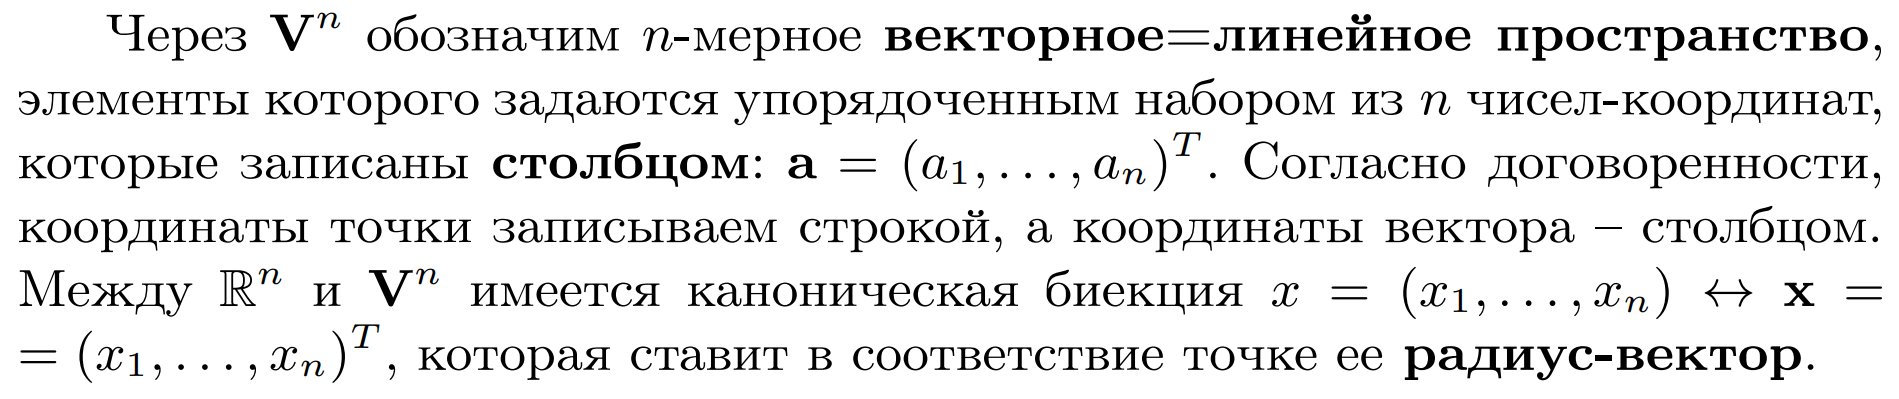
\includegraphics[width=\textwidth]{12.png}
    \vspace{-1cm}
\end{figure}
\begin{figure}[h!]
    \centering
    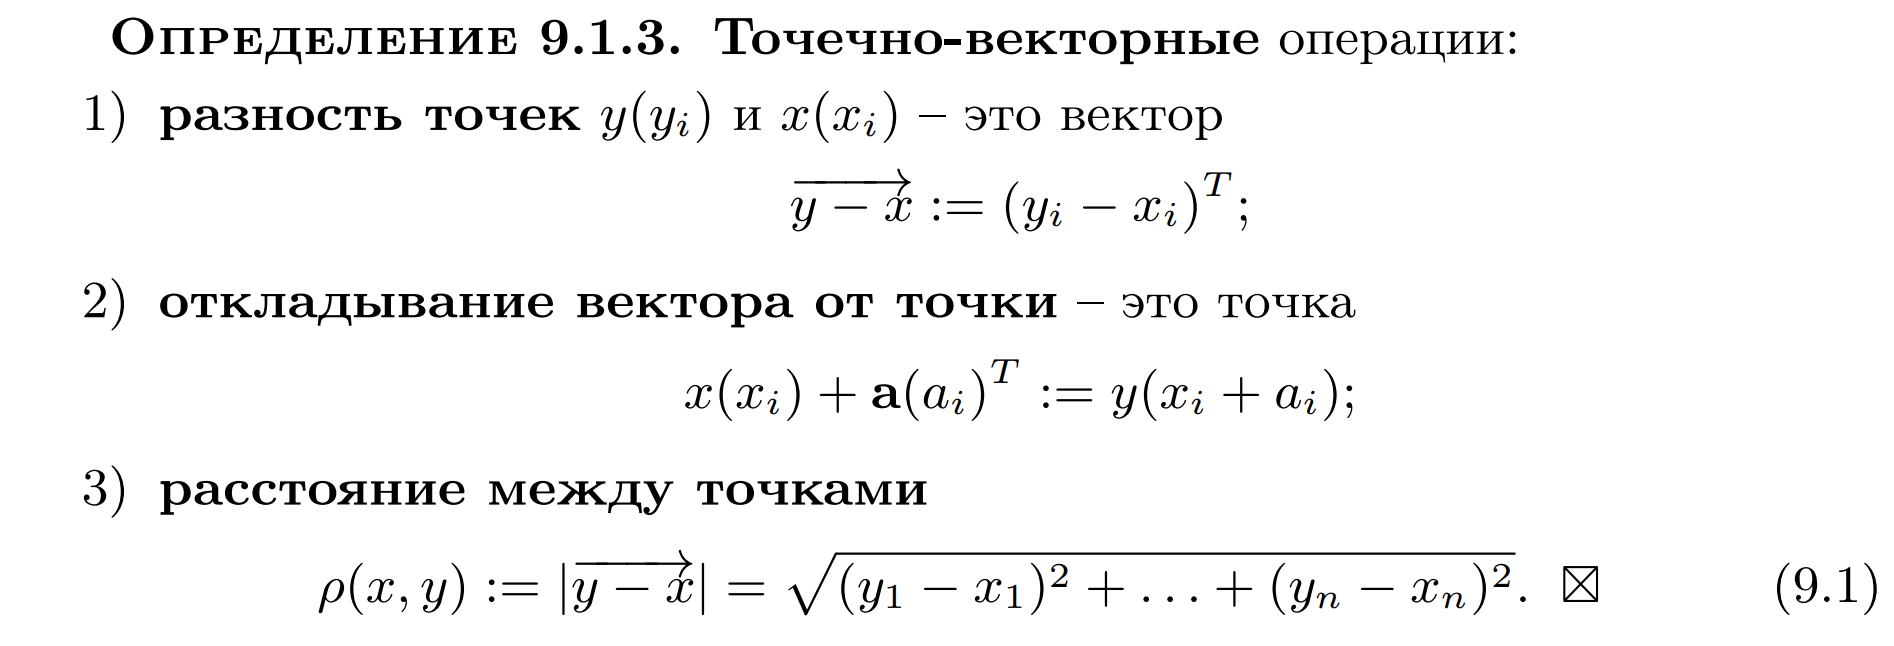
\includegraphics[width=\textwidth]{11.png}
    \vspace{-1cm}
\end{figure}
\begin{figure}[h!]
    \centering
    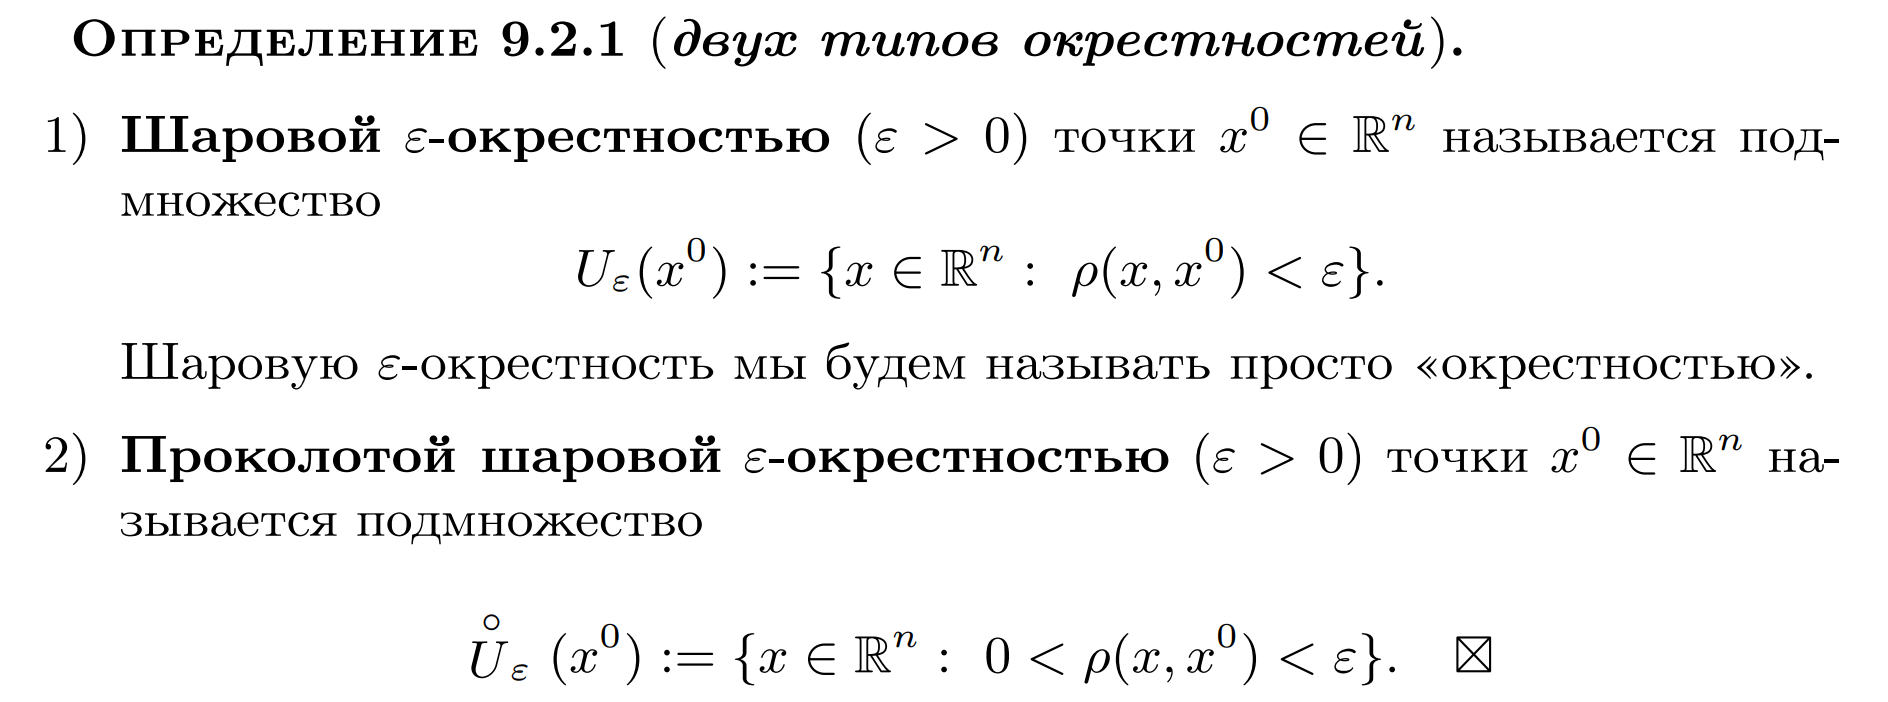
\includegraphics[width=\textwidth]{7.png}
    \vspace{-1cm}
\end{figure}
\newpage
\subsection{Предел последовательности точек в n-мерном пространстве.}
\begin{figure}[h!]
    \centering
    
\includegraphics[width=\textwidth]{2.png}
    \vspace{-1cm}
\end{figure}
\begin{figure}[h!]
    \centering
    \fbox{
\includegraphics[width=\textwidth]{3.png}}
    \vspace{-1cm}
\end{figure}
\newpage
\subsection{\ii{Связь между сходимостью последовательности точек и сходимостью последовательностей их координат.}}
\begin{figure}[h!]
    \centering
    \fbox{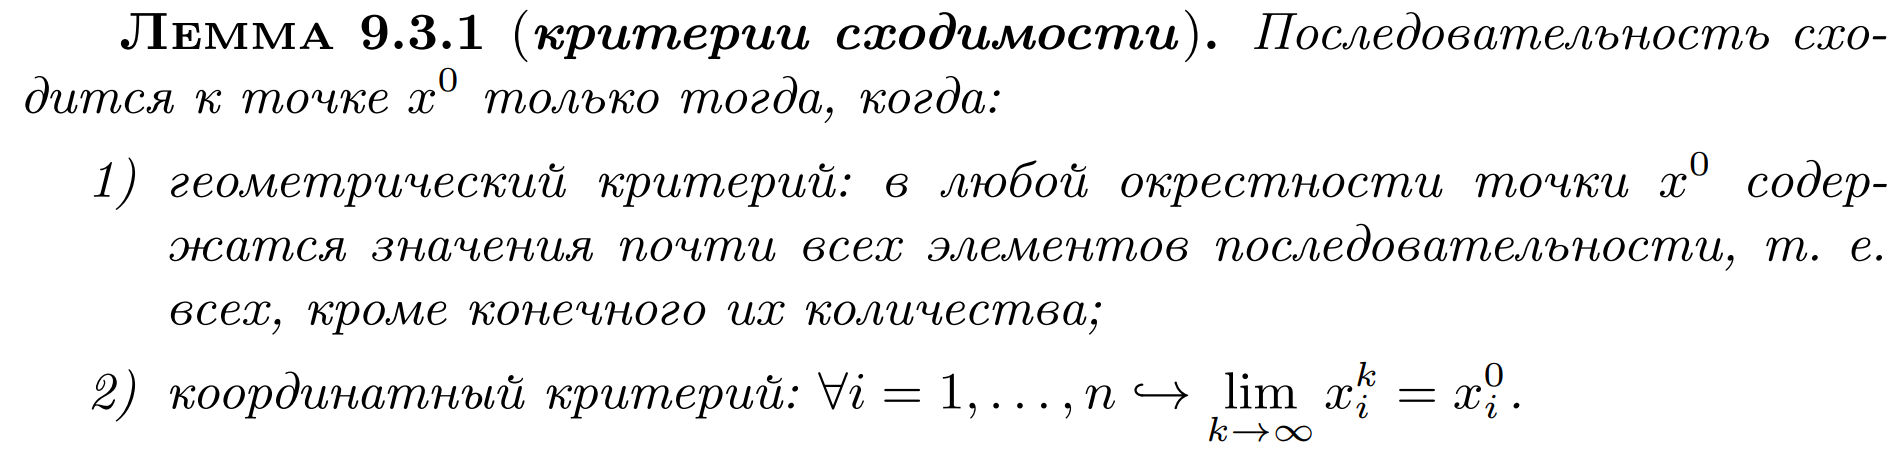
\includegraphics[width=\textwidth]{4.png}}
    \vspace{-1cm}
\end{figure}
\newpage
\subsection{Внутренние, предельные, изолированные точки множества.}
\begin{figure}[h!]
    \centering
    \fbox{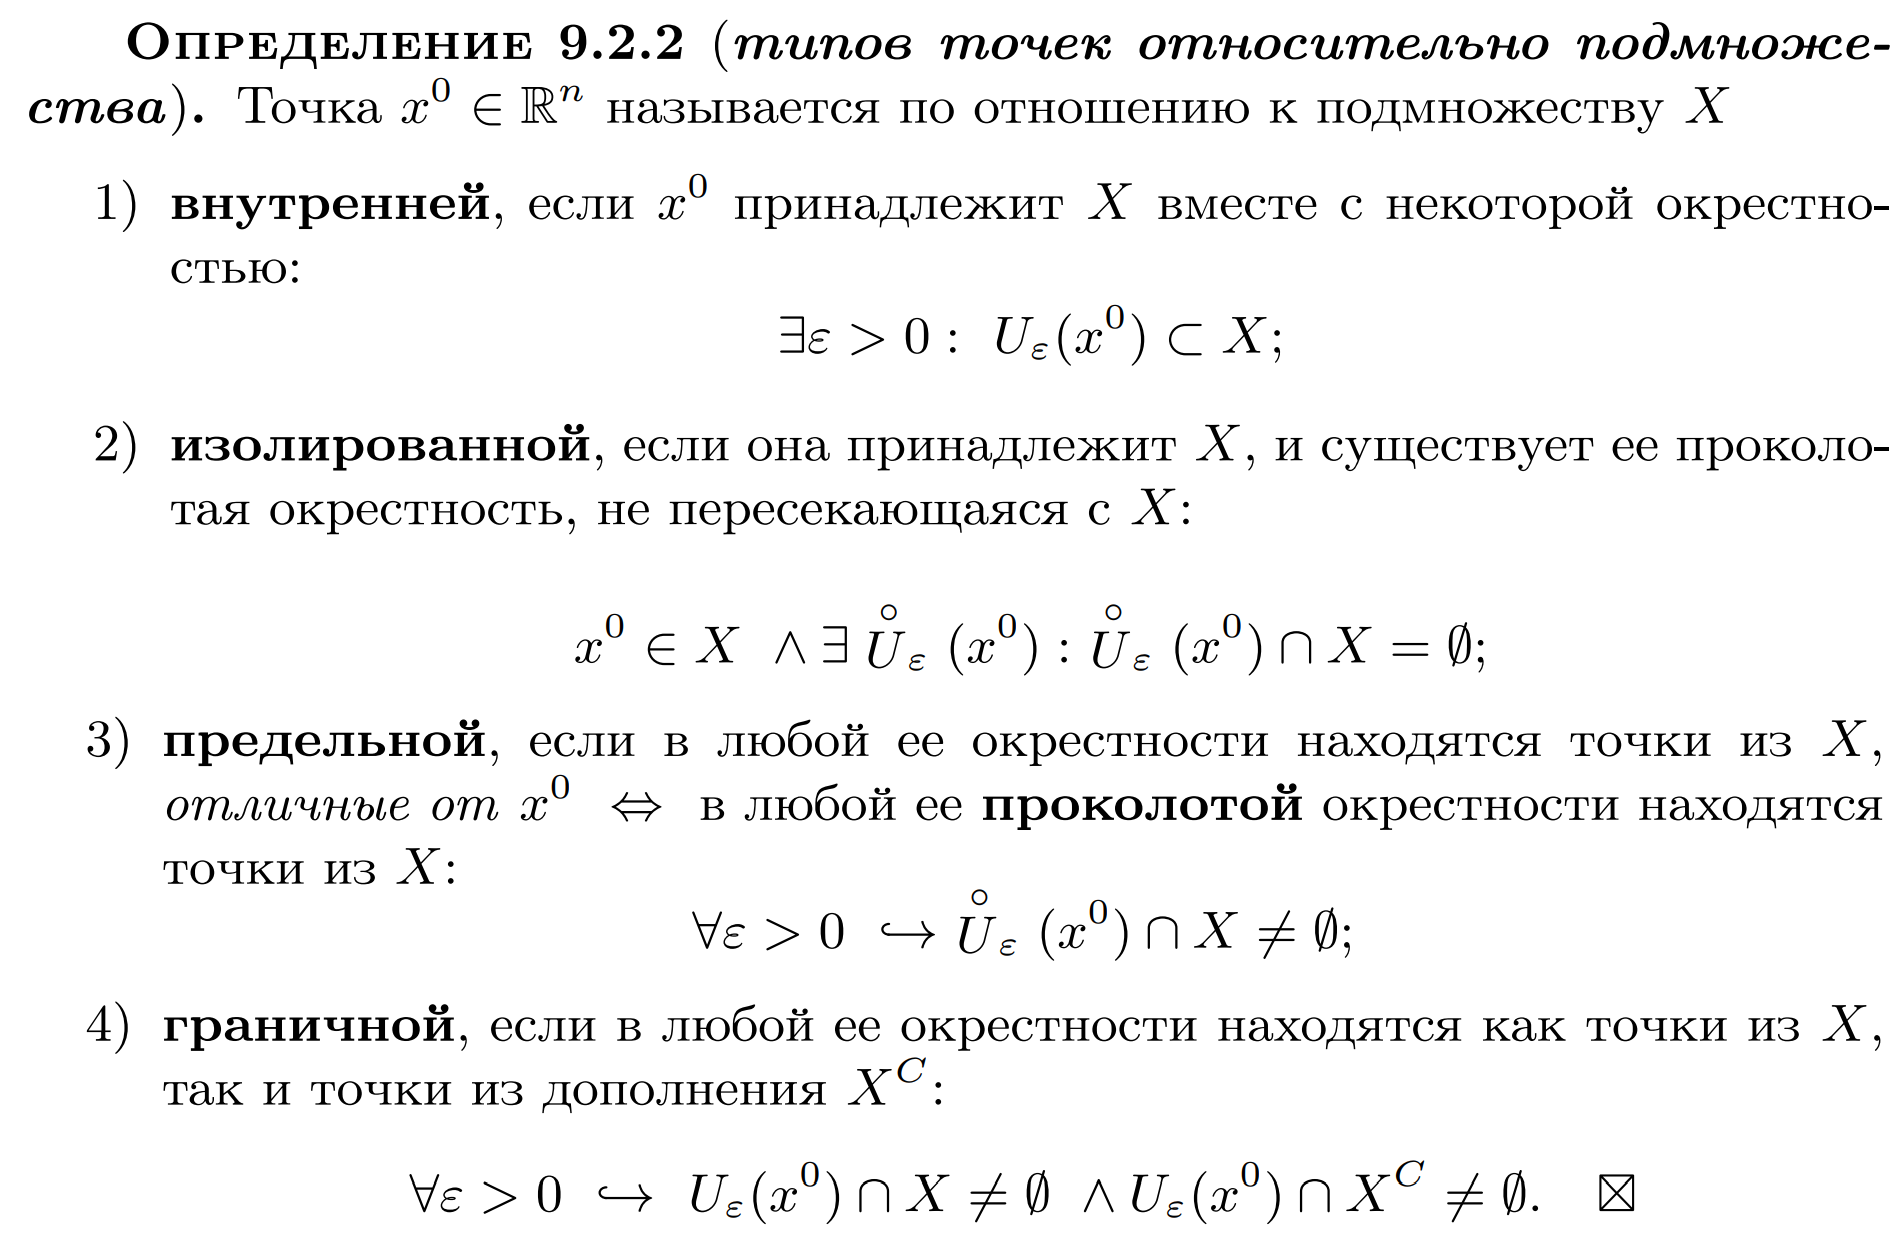
\includegraphics[width=\textwidth]{5.png}}
\end{figure}
{\bfseries\colorbox{lightgray}{Def}} $x_0$ называется точкой прикосновения множества $E$, если в любой её окресности найдутся точки из множества (не проколотой).

Изолированная точка является точкой прикосновения, но не является предельной, любая предельная является изолированной.

Изолированные точки обязательно принадлежат множеству, граничные могут не принадлежать ($(0,1)\cup \{2\}$ и концы $(0,1)$)
\begin{figure}[h!]
    \centering
    
\includegraphics[width=\textwidth]{8.png}
    \vspace{-1cm}
\end{figure}

{\bfseries\colorbox{lightgray}{Def}} (эквивалентное) $x^{0}$ -- предельная точка $E$, если $\exists x^{m} \to x^{(0)}, x^{m}\neq x^{(0)}$.

\newpage
\subsection{Открытые и замкнутые множества.}

\begin{figure}[h!]
    \centering
    \fbox{
\includegraphics[width=\textwidth]{9.png}}
\end{figure}

{\bfseries\colorbox{lightgray}{Def}} (альтернативные определения замкнутого множества) $M$ -- замкнуто, если оно содержит все свои граничные точки (точки прикосновения), (дополнение $\overline{M}$ открыто)

{\bfseries\colorbox{lightgray}{Def}} \bb{Область} -- открытое, линейно связное множество.

{\bfseries\colorbox{lightgray}{Def}} $E$ -- \bb{линейно связное множество}, если $\forall x_1, x_2 \in E$ можем соединить кривойБ принадлежащей $E$

{\bfseries\colorbox{lightgray}{Def}} \bb{Компакт} -- ограниченное, замкнутое множество.

{\bfseries\colorbox{lightgray}{Def}} $E$ -- ограничено, если $\exists U_\varepsilon(0) : E\subset U_\varepsilon(0)$

\begin{figure}[h!]
    \centering
    \fbox{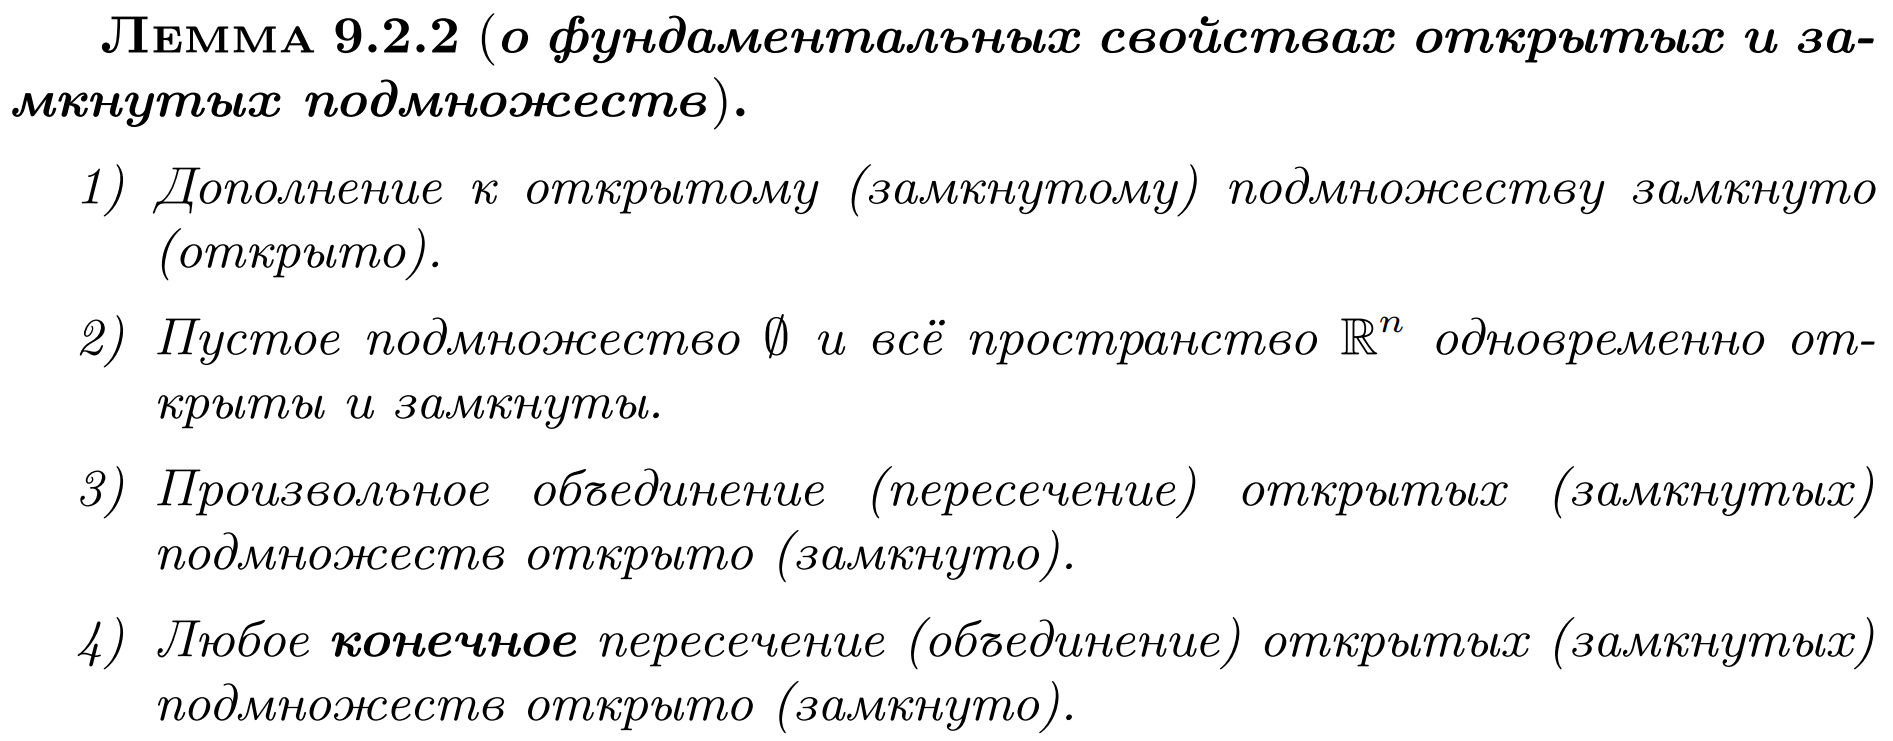
\includegraphics[width=\textwidth]{10.png}}
    \vspace{-1cm}
\end{figure}
\subsection{Внутренность, замыкание и граница множества.}
\begin{figure}[h!]
    \centering
    \fbox{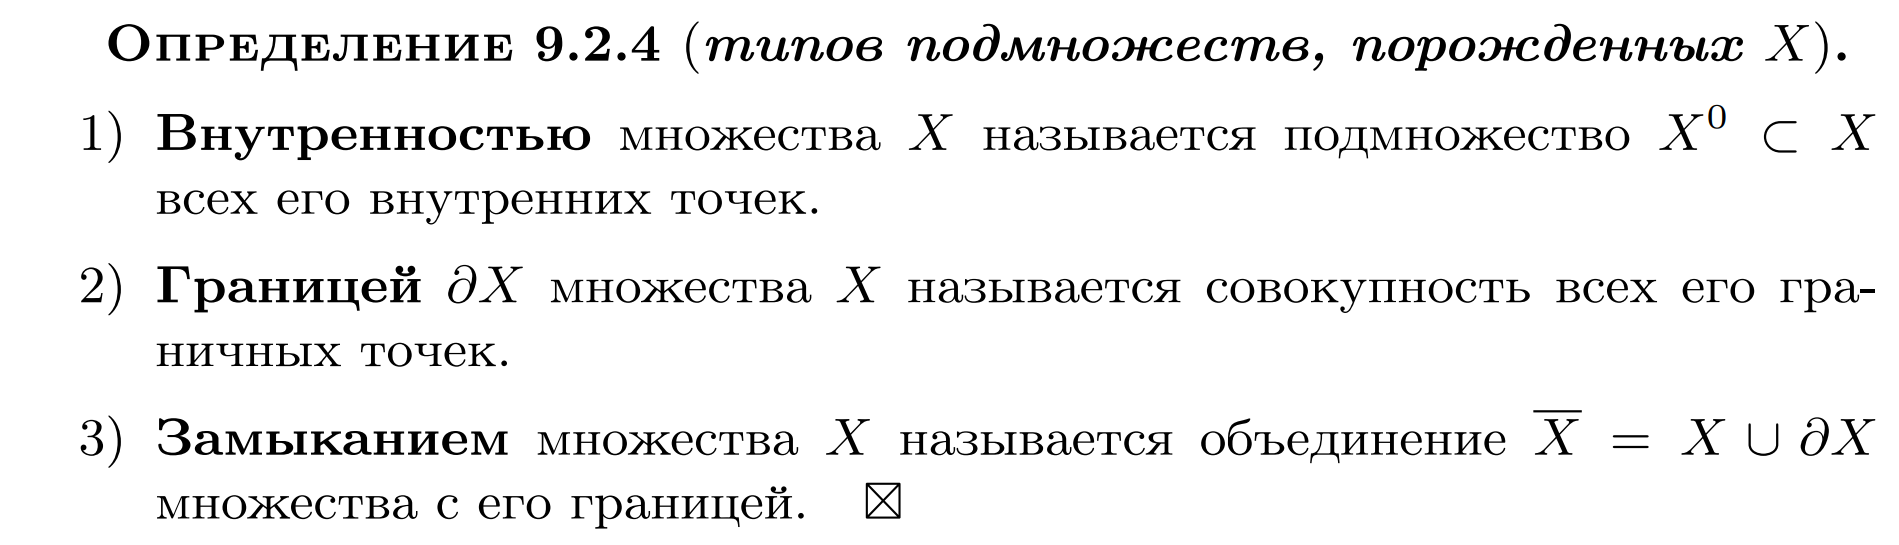
\includegraphics[width=\textwidth]{13.png}}
    \vspace{-1cm}
\end{figure}
\newpage\noindent
\bb{Summary}

\ii{Внутренняя точка} -- лежит в множестве вместе с окрестностью

\ii{Изолированная точка} -- существует проколотая окрестность, не содержащая точек множества

\ii{Предельная точка} -- точка, в любой проколотой окрестности которой есть точки из множества или есть последовательность Гейне, принадлежащая множеству

\ii{Граничная точка} -- любая окрестность содержит точки из множества и дополнения.

\ii{Точка прикосновения} -- в любой окрестности (не проколотой) есть точки из множества.

\ii{Открытое множество} -- все его точки внутренние.

\ii{Замкнутое множество} -- содержит все предельные точки, дополнение открыто, сожержит все граничные точки, точки прикосновения.

\ii{Область} -- открытое множество, точки которого можно соединить кривой (не обязательно гладкой), принадлежащей множеству.

\ii{Компакт} -- замкнутое множество, принадлежащее некоторой окрестности нуля.

\ii{Th} Пересечение конечного количества открытых множеств открыто.

\ii{Th} Объединение любого количества открытых множеств открыто.

\ii{Th} Аналогично с замкнутыми множествами.

\ii{Внутренность} -- множество всех внутренних точек.

\ii{Граница} -- множество всех граничных точек.

\ii{Замыкание} -- объединение множества с его границей.

\newpage\noindent
%\section{\color{RedViolet}\textbf{Предел числовой функции нескольких переменных. Предел функции по множеству. Пределы по направлениям. Непрерывность функции нескольких переменных в точке и по множеству. Непрерывность сложной функции. Свойства функций, непрерывных на компакте — ограниченность, достижимость (точных) нижней и верхней граней, равномерная непрерывность. Теорема о промежуточных значениях функции, непрерывной в области.}}
\section{Пределы, непрерывность функций нескольких переменных.}
\begin{figure}[h!]
    \centering
    
\includegraphics[width=\textwidth]{14.png}
    \vspace{-1cm}
\end{figure}
\subsection{Предел функции нескольких переменных.}
\begin{figure}[h!]
    \centering
    \fbox{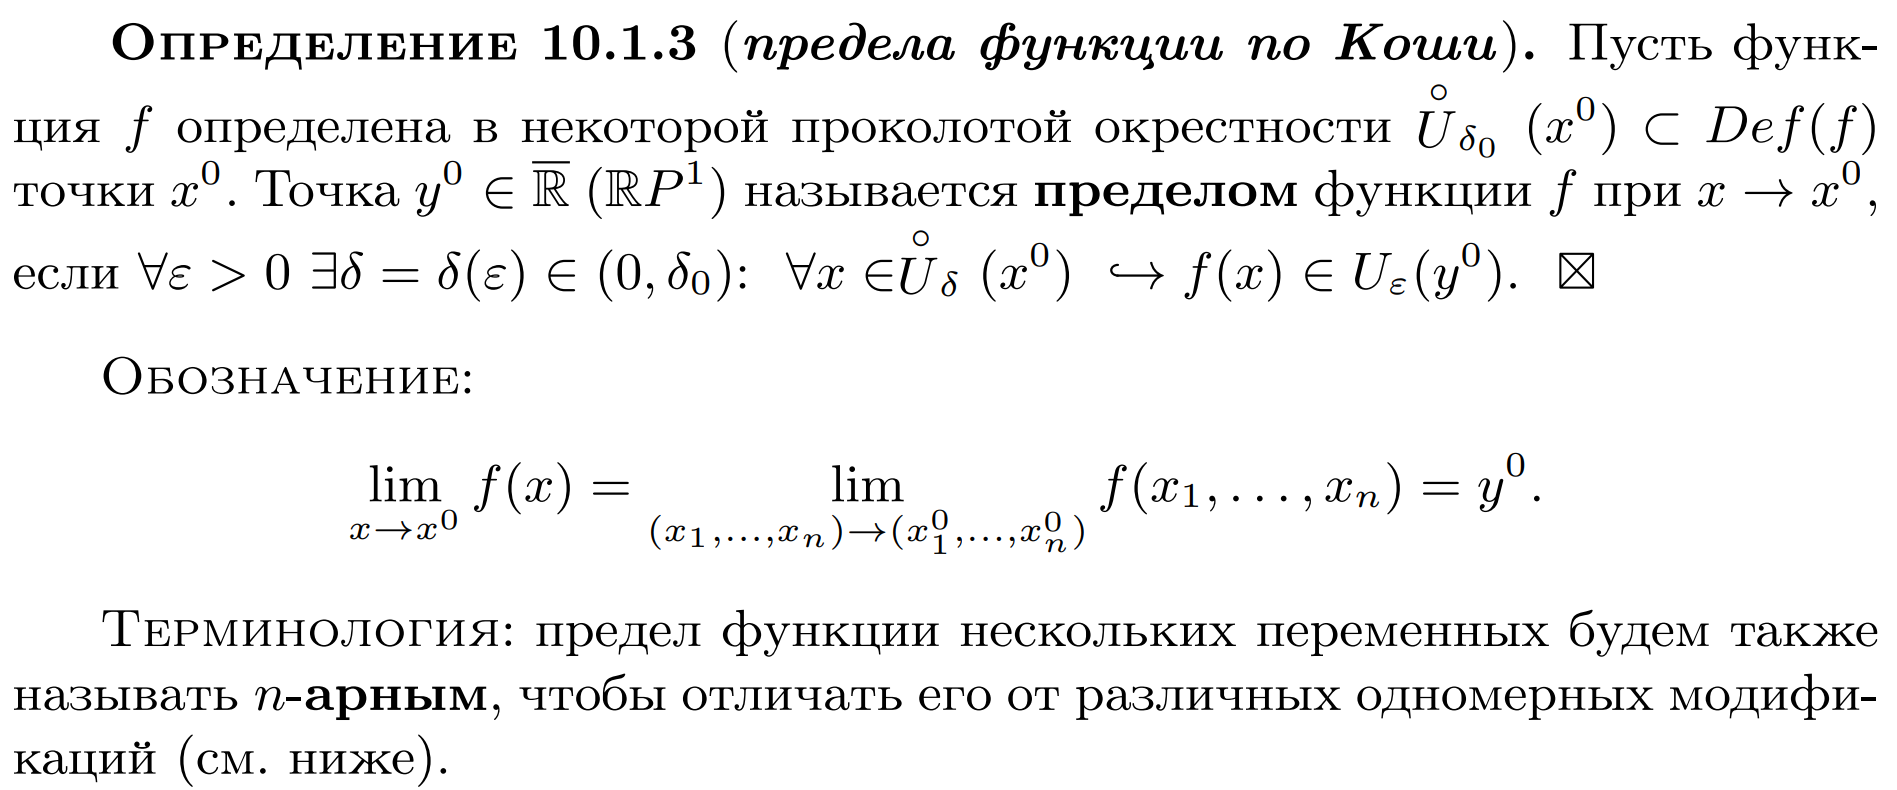
\includegraphics[width=\textwidth]{15.png}}
    \vspace{-1cm}
\end{figure}
\begin{figure}[h!]
    \centering
    \fbox{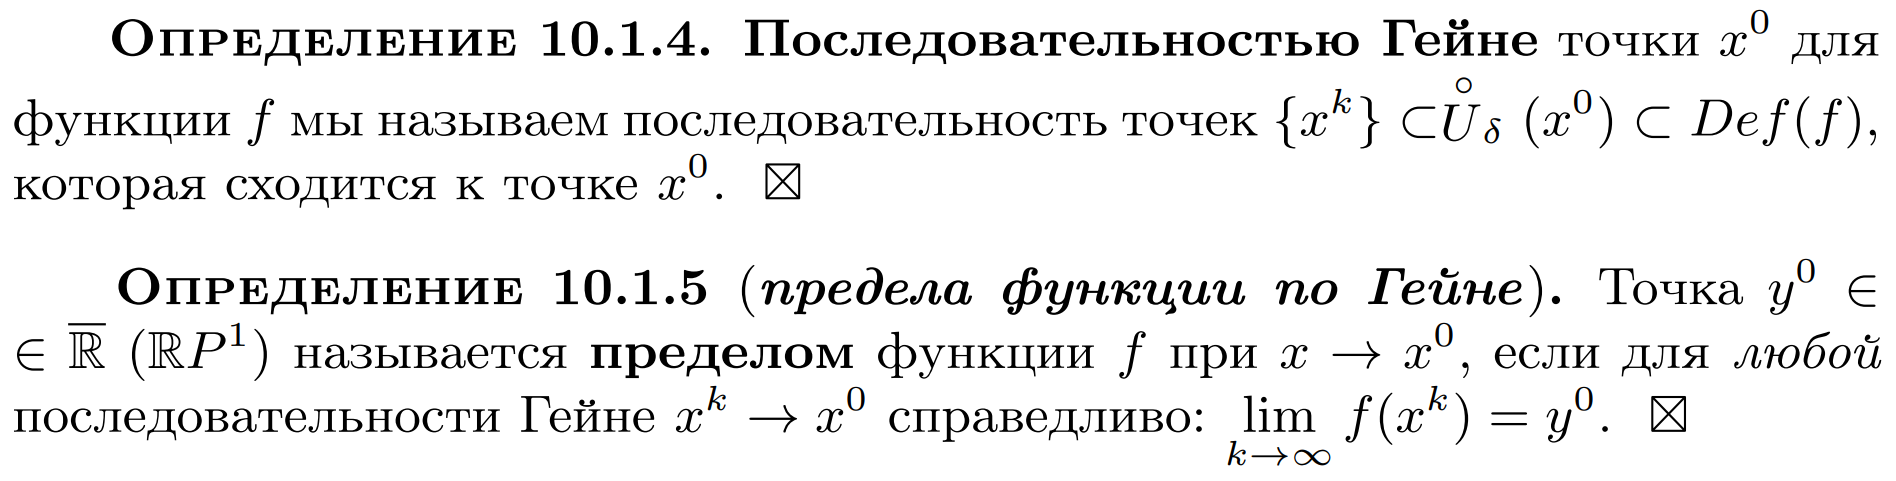
\includegraphics[width=\textwidth]{16.png}}
\end{figure}

% {\bfseries\colorbox{lightgray}{Def}} \bb{Повторный предел} -- сначала берём предел по одной переменной, а потом по второй, рассматривая предел по первой как функцию.
% $$\lim\limits_{y\to 0}\lim\limits_{x\to 0} \left( x+y \sin\frac{1}{x} \right) = \emptyset$$title
% $$\lim\limits_{x\to 0}\lim\limits_{y \to 0}\left( x + y \sin \frac{1}{x} \right) = 0 $$

% \newpage
% \begin{figure}[h!]
%     \centering
%     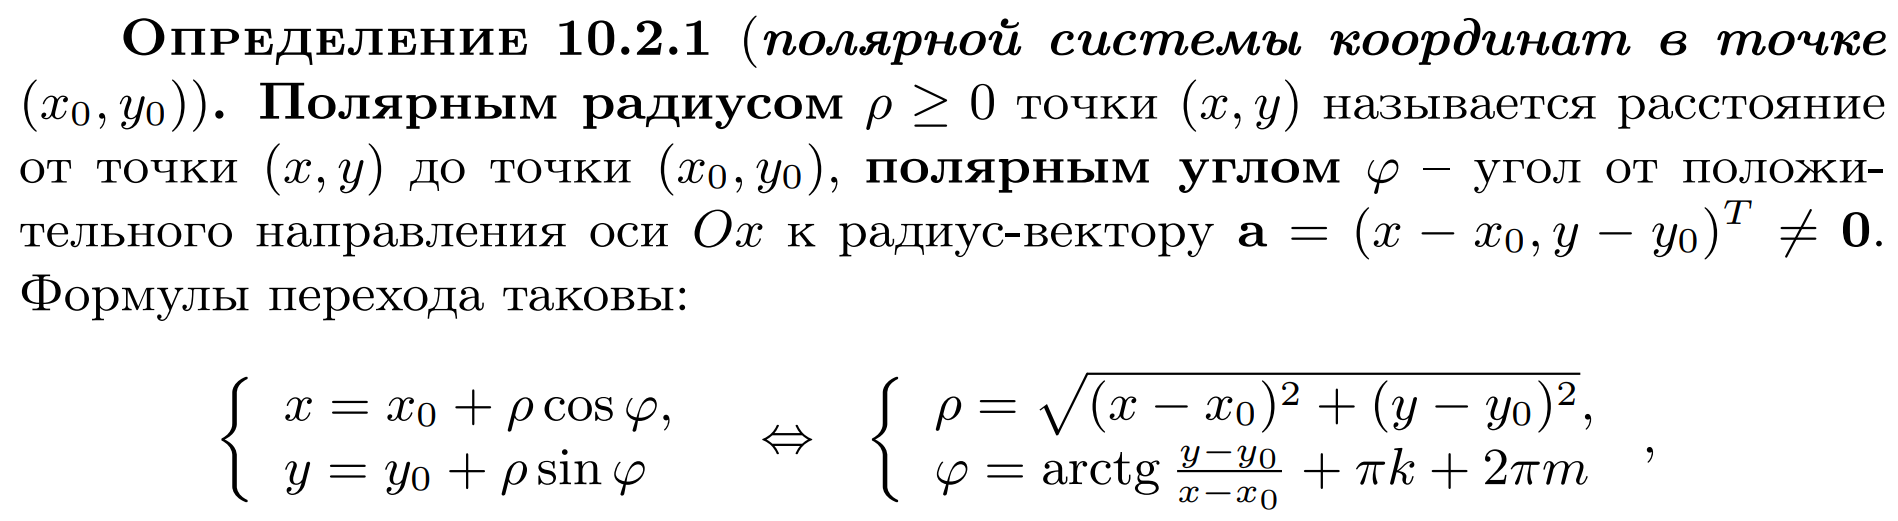
\includegraphics[width=\textwidth]{17.png}
%     \vspace{-1cm}
% \end{figure}
% \begin{figure}[h!]
%     \centering
%     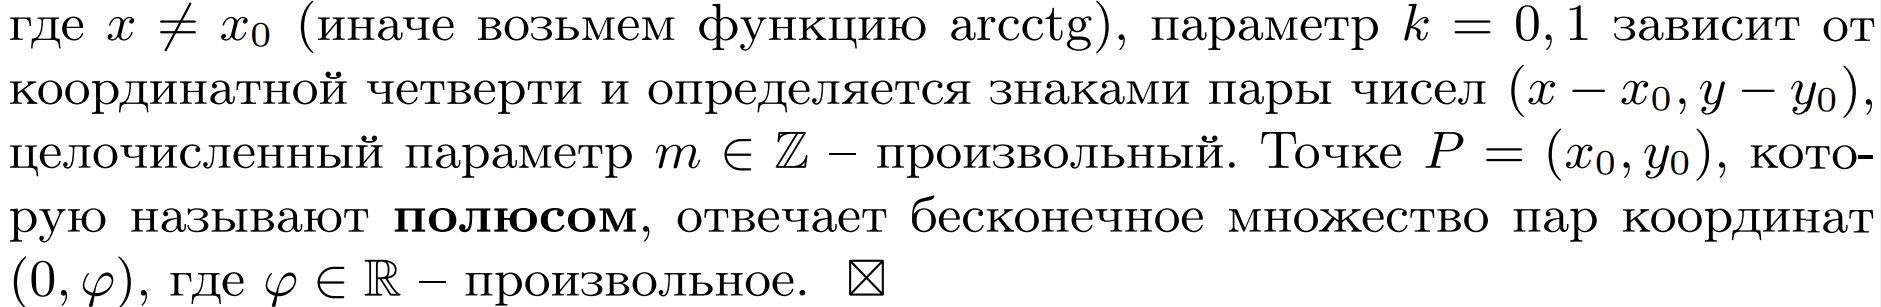
\includegraphics[width=\textwidth]{18.png}
%     \vspace{-1cm}
% \end{figure}

\newpage
\subsection{Предел по направлению}
\begin{figure}[h!]
    \centering
    \fbox{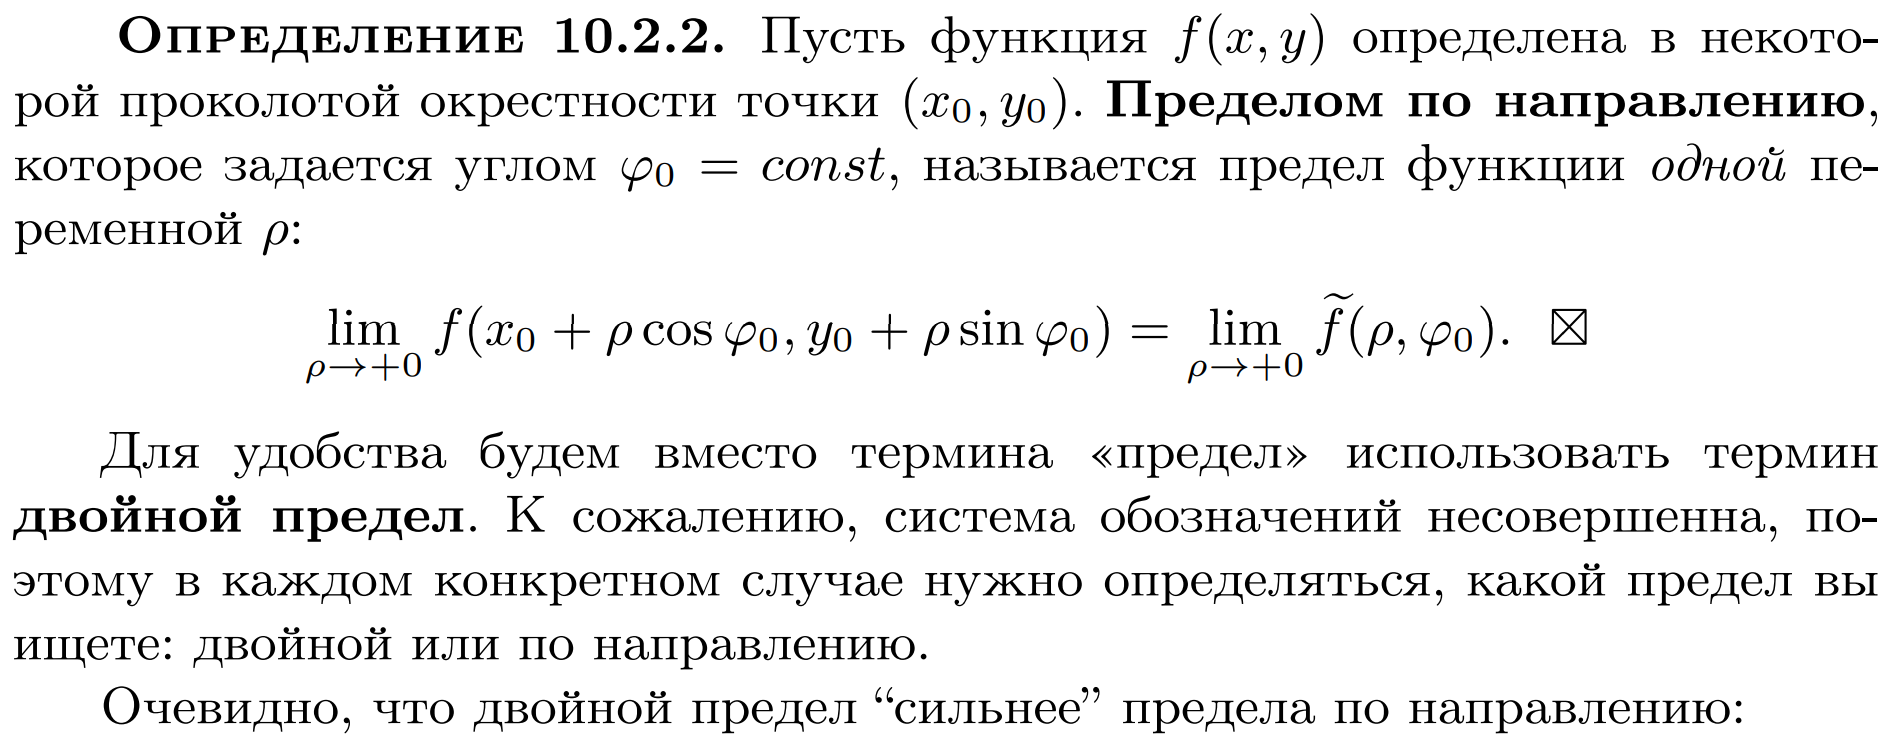
\includegraphics[width=\textwidth]{19.png}}
    \vspace{-1cm}
\end{figure}
\begin{figure}[h!]
    \centering
    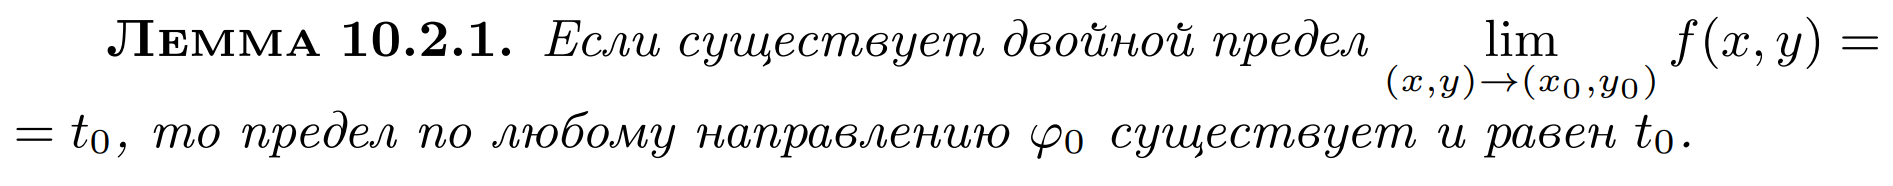
\includegraphics[width=\textwidth]{20.png}
    \vspace{-1cm}
\end{figure}
\begin{figure}[h!]
    \centering
    
\includegraphics[width=\textwidth]{41.png}
    \vspace{-1cm}
\end{figure}
\paragraph*{Лемма} $\exists \lim\limits_{x\to x^0}f(x) = y^0 \Rightarrow \forall \mathbf{e} \; \exists \lim\limits_{\rho \to 0}f_{\mathbf{e}}(\rho)=y_0$

\newpage
\subsection{Предел функции по множеству.}
\begin{figure}[h!]
    \centering
    \fbox{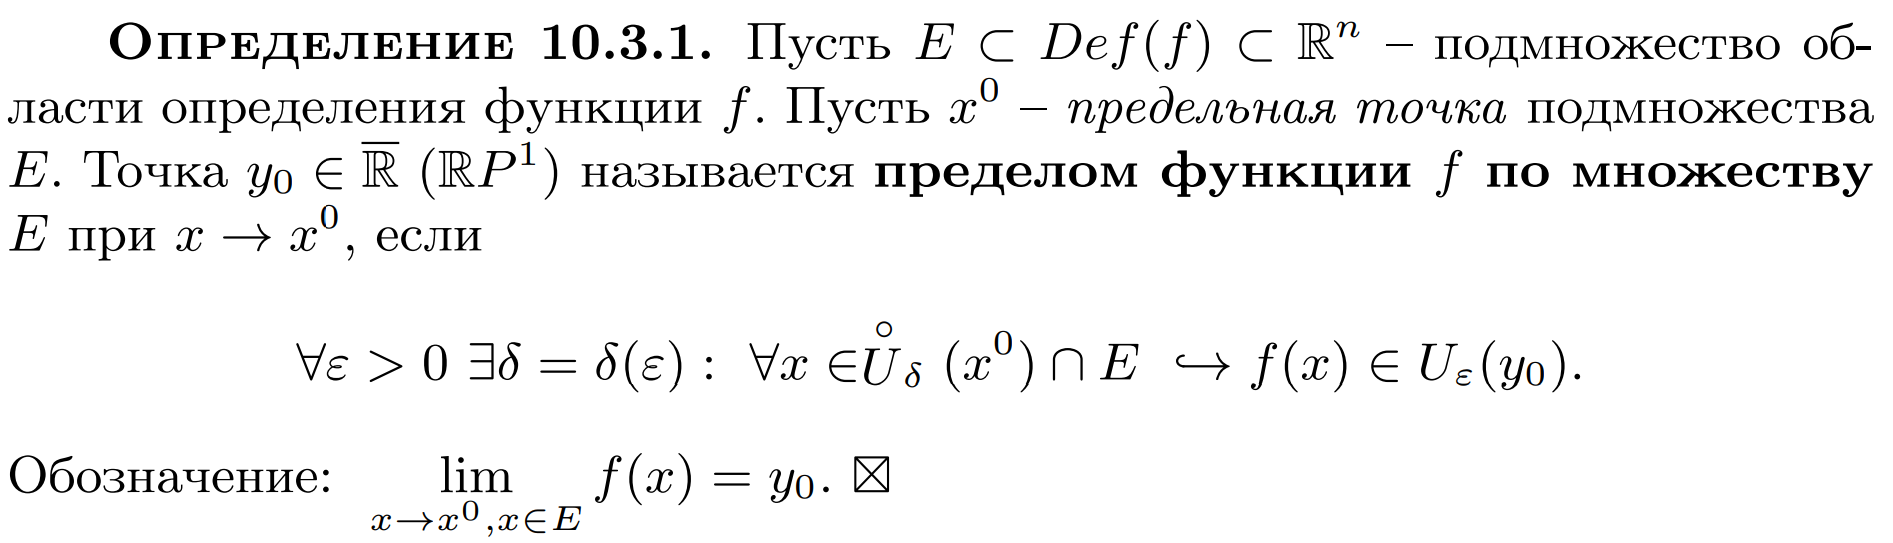
\includegraphics[width=\textwidth]{21.png}}
\end{figure}
Например, односторонние пределы функции одной переменной или предел по направлению функции нескольких переменных.

{\bfseries\colorbox{lightgray}{Def}} (Скубачевский) Предел по направлению -- предел по множеству $E$, где $E$ -- луч.

\bb{Утв} $\exists \lim\limits_{x\to x^{(0)}} f(x) \Rightarrow$ в точке $x^{(0)}$ существует предел по всем направлениям, и они равны.

Обратное не верно. Пример: парабола, поднятая вверх на 1 для точки (0,0).
\newpage
\subsection{Непрерывность функции нескольких переменных в точке и по множеству.}
\begin{figure}[h!]
    \centering
    \fbox{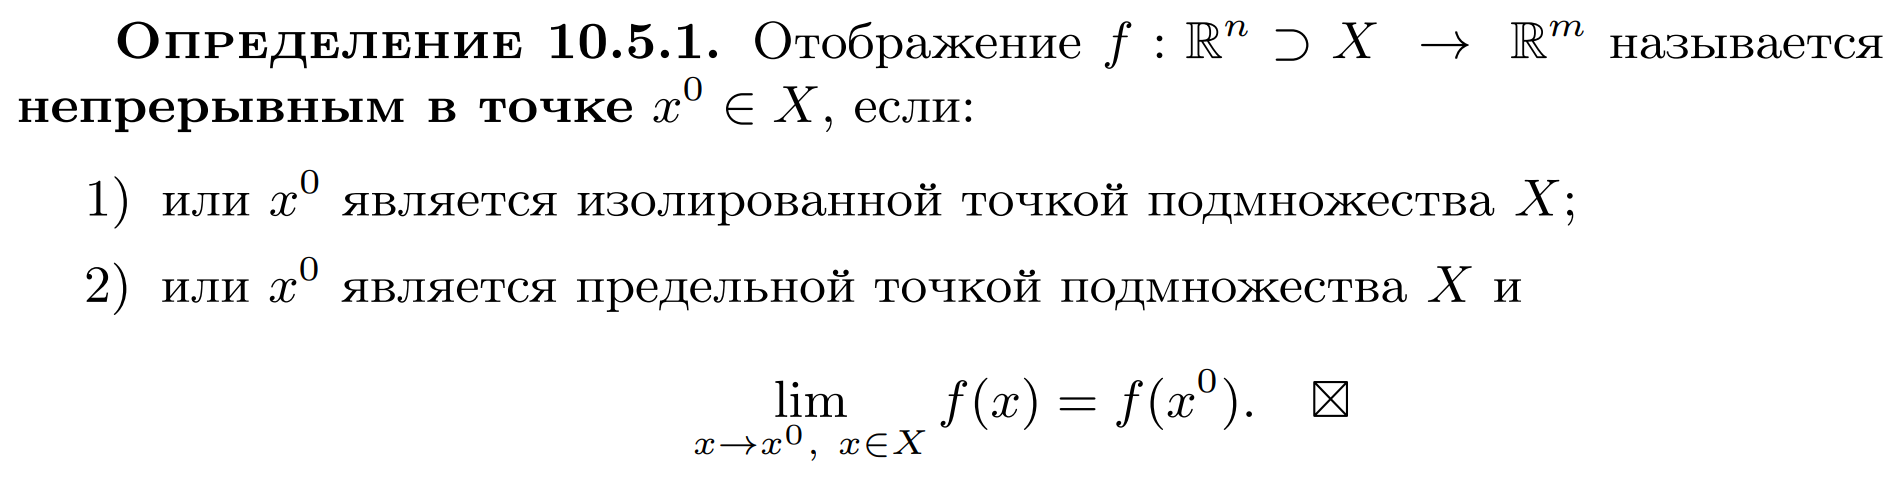
\includegraphics[width=\textwidth]{22.png}}
    \vspace{-1cm}
\end{figure}
\begin{figure}[h!]
    \centering
    \fbox{
\includegraphics[width=\textwidth]{29.png}}
    \vspace{-1cm}
\end{figure}
\begin{figure}[h!]
    \centering
    \fbox{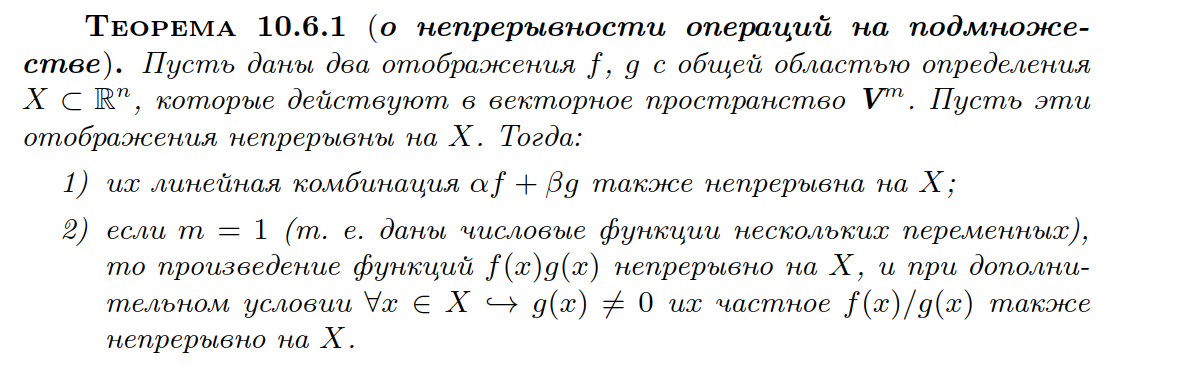
\includegraphics[width=\textwidth]{42.png}}
    \vspace{-1cm}
\end{figure}
\begin{figure}[h!]
    \centering
    \fbox{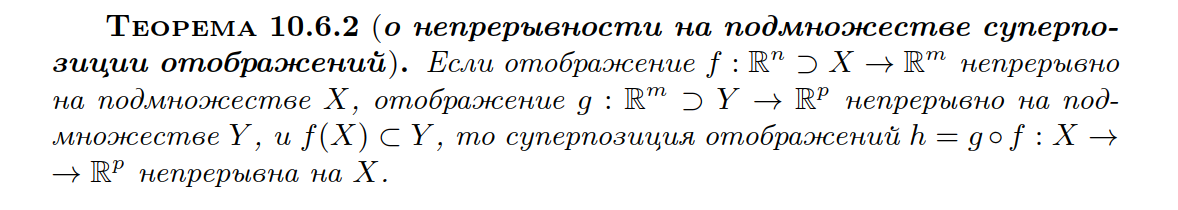
\includegraphics[width=\textwidth]{43.png}}
    \vspace{-1cm}
\end{figure}
\begin{figure}[h!]
    \centering
    \fbox{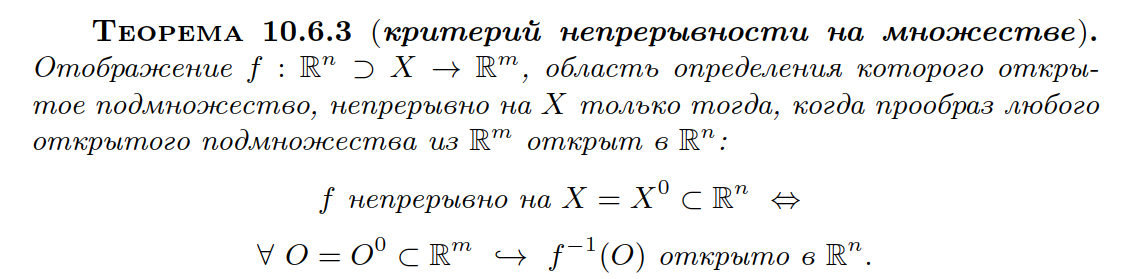
\includegraphics[width=\textwidth]{44.png}}
    \vspace{-1cm}
\end{figure}
\begin{figure}[h!]
    \centering
    \fbox{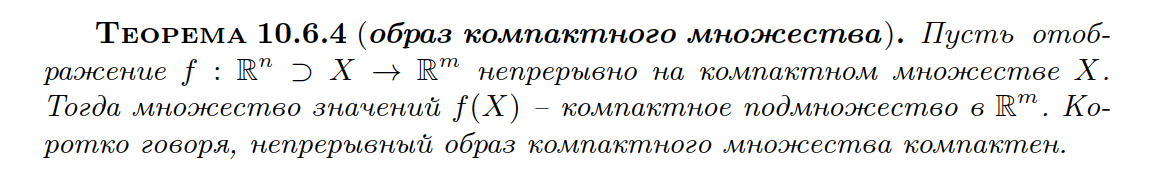
\includegraphics[width=\textwidth]{45.png}}
    \vspace{-1cm}
\end{figure}
\begin{figure}[h!]
    \centering
    \fbox{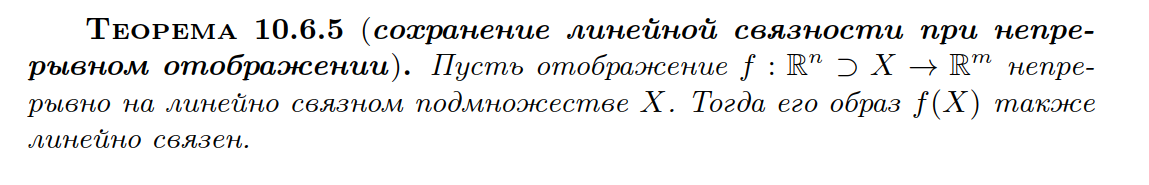
\includegraphics[width=\textwidth]{46.png}}
    \vspace{-1cm}
\end{figure}


\paragraph*{Пример:} Исследовать $f(x,y)$ на непрерывность в точке (0,0).
$$f(x,y) = \frac{2xy}{\sqrt{x^2+y^2}}$$
По теореме о трёх милиционерах:
$$0 \leq |f(x,y)| = \left| \frac{2xy}{\sqrt{x^2 + y^2}} \right| = \left| \frac{2 \rho^2 \sin\varphi \cos\varphi}{\rho} \right| \leq 2\rho \to 0$$
\ii{Второй милиционер не должен зависеть от $\varphi$!}
% \begin{figure}[h!]
%     \centering
%     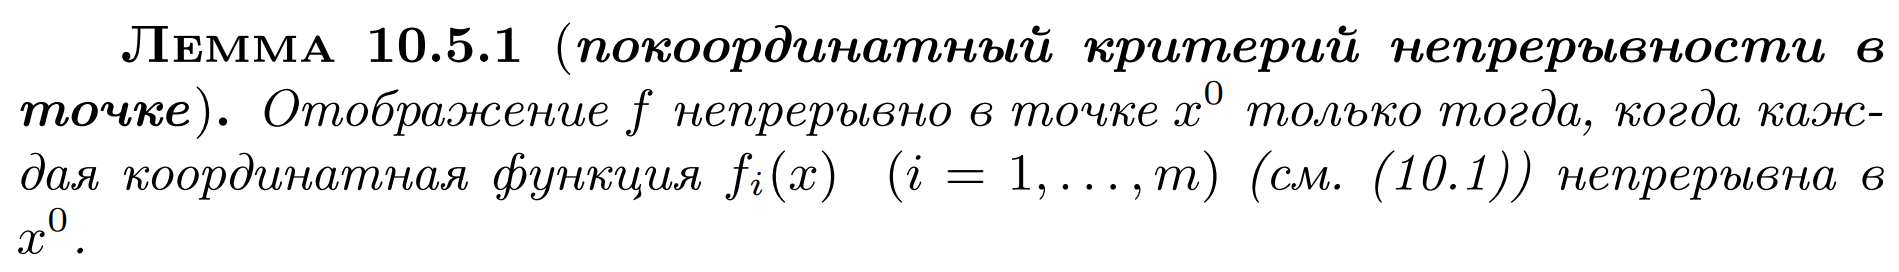
\includegraphics[width=\textwidth]{23.png}
%     \vspace{-1cm}
% \end{figure}
% \begin{figure}[h!]
%     \centering
%     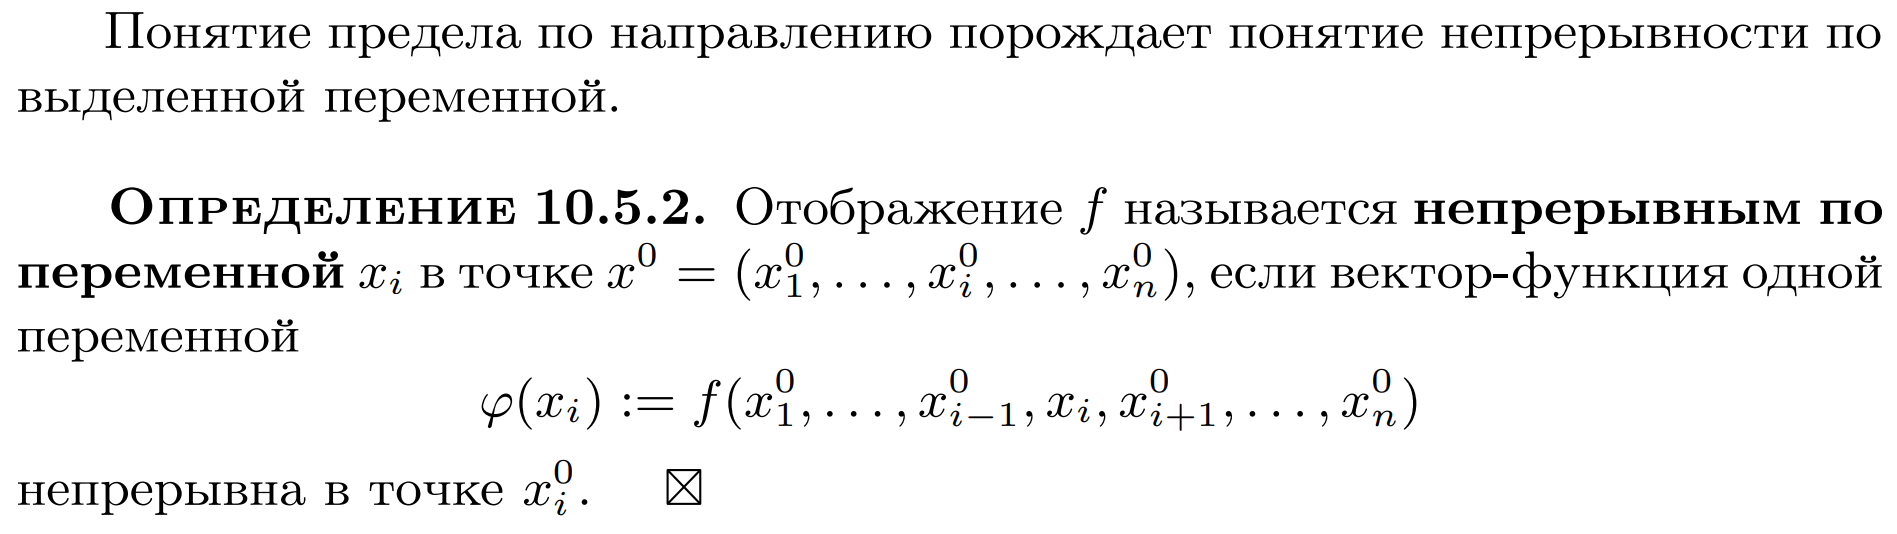
\includegraphics[width=\textwidth]{24.png}
%     \vspace{-1cm}
% \end{figure}
% \newpage
% \begin{figure}[h!]
%     \centering
%     
\includegraphics[width=\textwidth]{25.png}
%     \vspace{-1cm}
% \end{figure}
% \begin{figure}[h!]
%     \centering
%     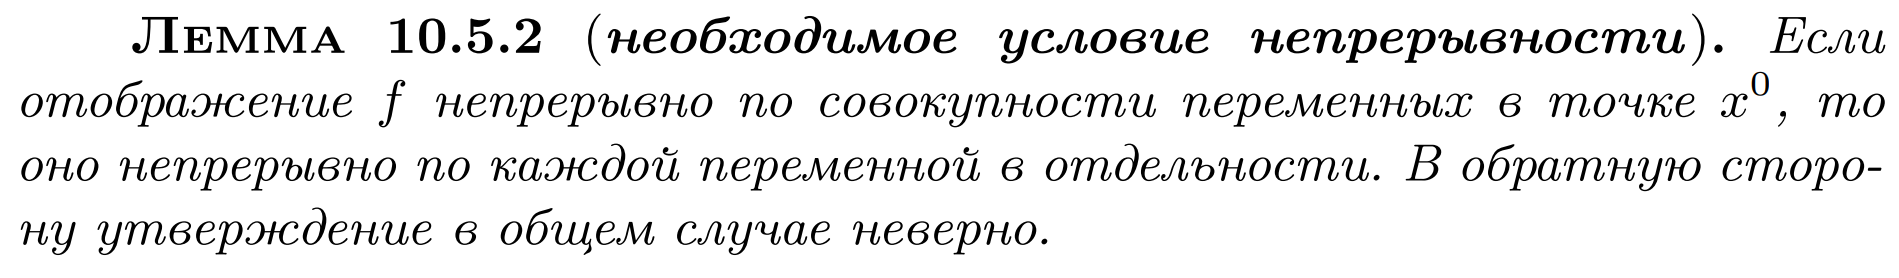
\includegraphics[width=\textwidth]{26.png}
%     \vspace{-1cm}
% \end{figure}
% \begin{figure}[h!]
%     \centering
%     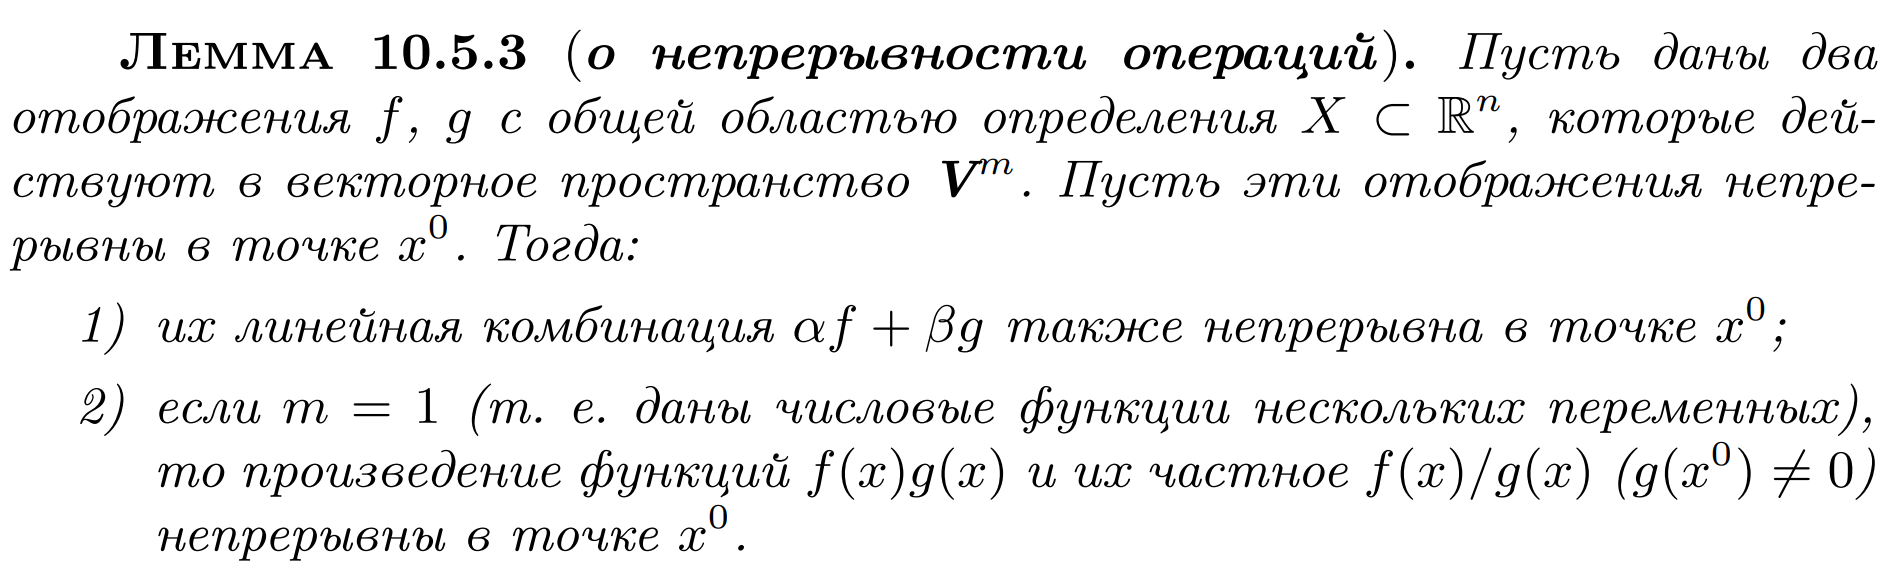
\includegraphics[width=\textwidth]{27.png}
%     \vspace{-1cm}
% \end{figure}
\newpage
\subsection{Непрерывность сложной функции}
\begin{figure}[h!]
    \centering
    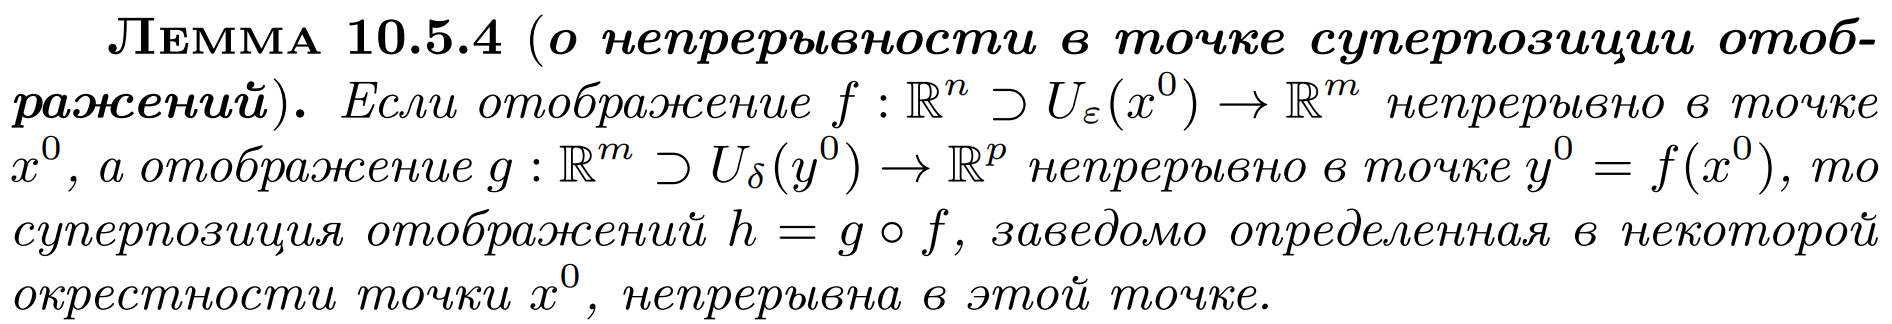
\includegraphics[width=\textwidth]{28.png}
    \vspace{-1cm}
\end{figure}
% \newpage
% \begin{figure}[h!]
%     \centering
%     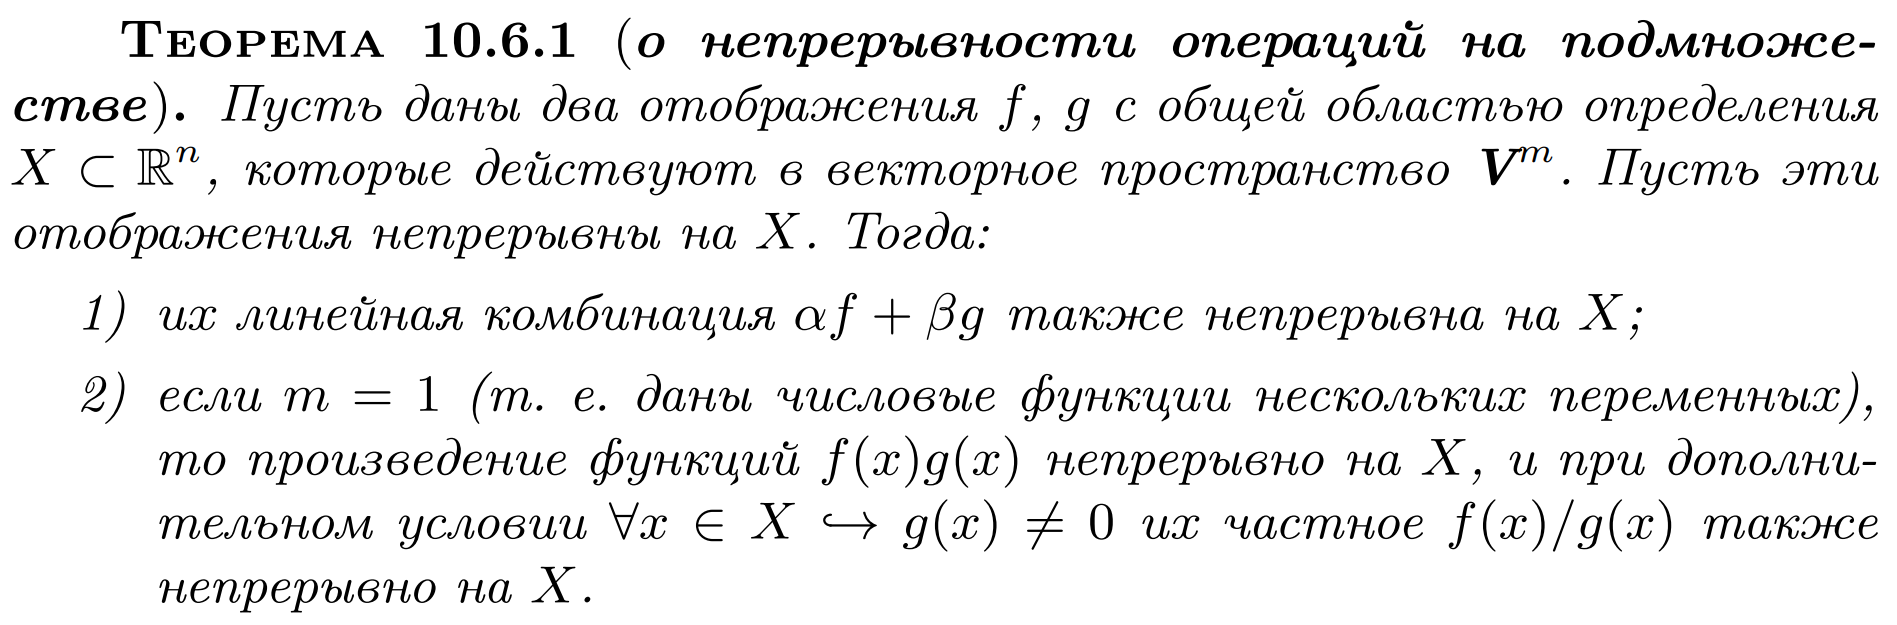
\includegraphics[width=\textwidth]{30.png}
%     \vspace{-1cm}
% \end{figure}
% \begin{figure}[h!]
%     \centering
%     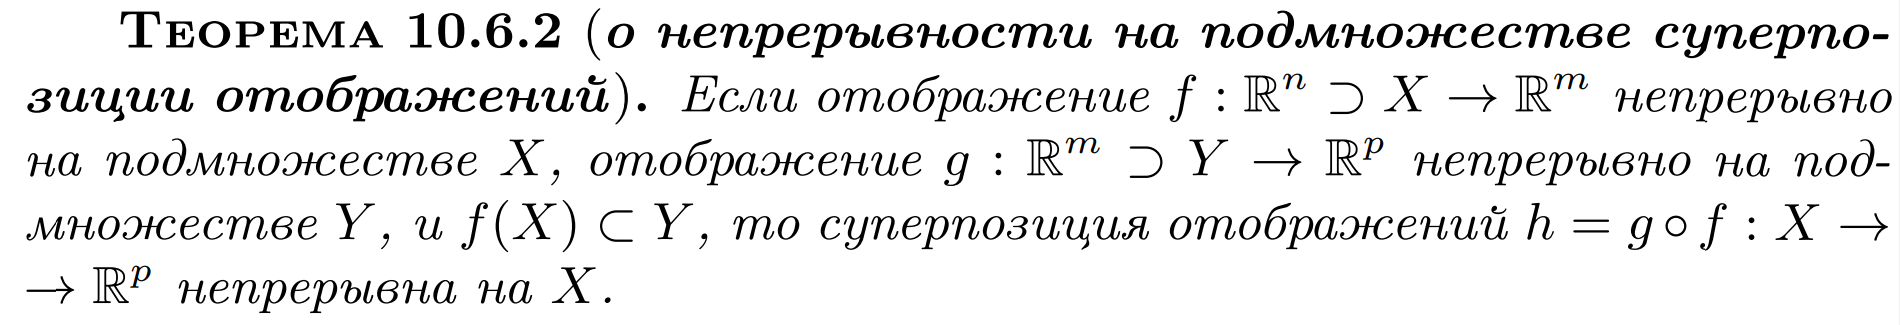
\includegraphics[width=\textwidth]{31.png}
%     \vspace{-1cm}
% \end{figure}
% \newpage
% \begin{figure}[h!]
%     \centering
%     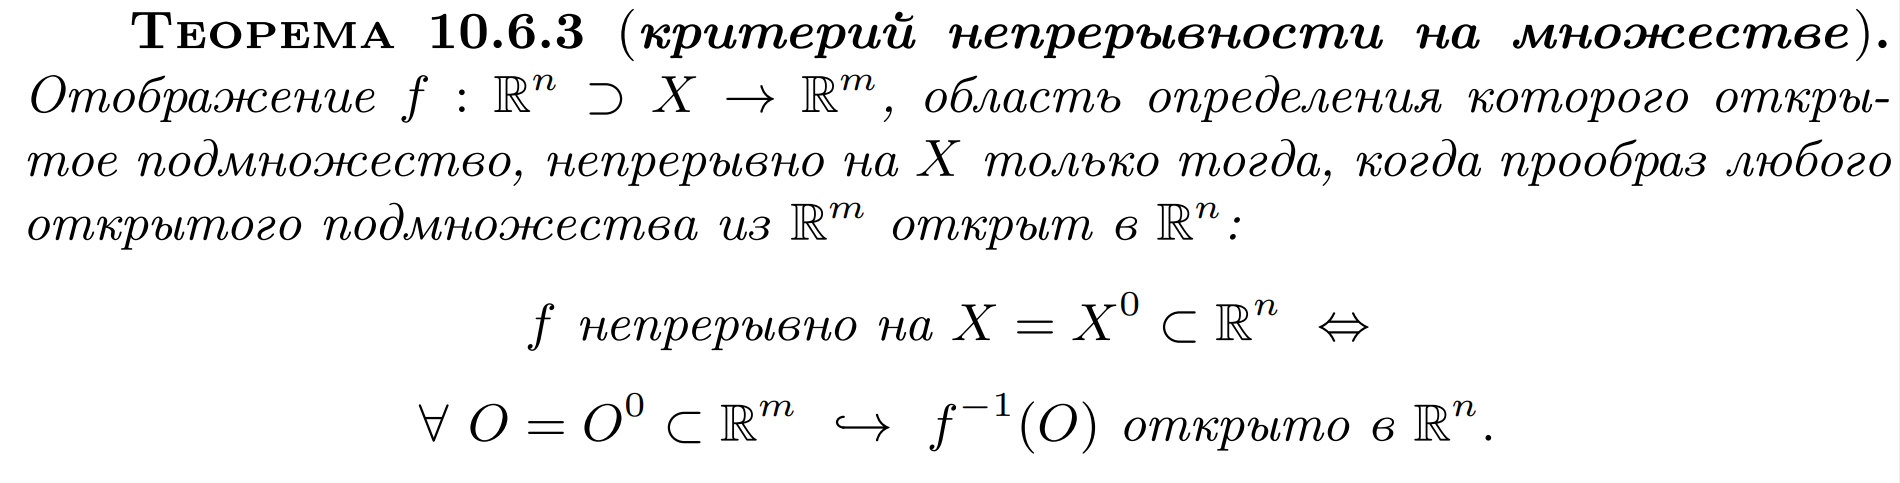
\includegraphics[width=\textwidth]{32.png}
%     \vspace{-1cm}
% \end{figure}


\newpage
\subsection{Свойства функций, непрерывных на компакте -- ограниченность, достижимость (точных) нижней и верхней граней, равномерная непрерывность.}
\begin{figure}[h!]
    \centering
    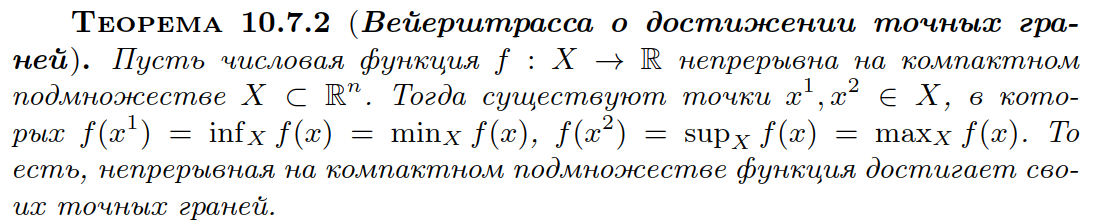
\includegraphics[width=\textwidth]{47.png}
    \vspace{-1cm}
\end{figure}
\begin{figure}[h!]
    \centering
    
\includegraphics[width=\textwidth]{48.png}
\end{figure}
\underline{\bb{Опр}}
$$f: \R^n \supset X \to \R^m $$
$f$ равномерно непрерывна на $X$, если
$$ \forall \varepsilon > 0 \; \exists \delta > 0 : \forall x', x'' \in X : \rho(x',x'') < \delta \hookrightarrow \rho(f(x'). f(x'')) < \varepsilon $$
\newpage
\subsection{Теорема о промежуточных значениях функции, непрерывной в области.}
\begin{figure}[h!]
    \centering
    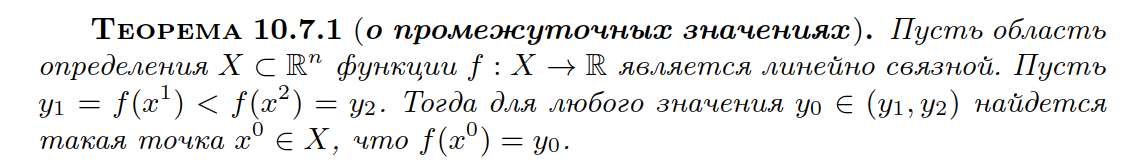
\includegraphics[width=\textwidth]{49.png}
    \vspace{-1cm}
\end{figure}
\newpage
\subsection{Не вошло в программу экзамена.}
\subsubsection{Повторный предел}
\bb{Опр} $f: \Pi_\varepsilon(x_0, y_0) \to \R $. $\Pi$ -- Декартово произведение окрестностей $x_0$ и $y_0$. \\
Пусть $\forall y \in \mathring{U}(y_0)\hookrightarrow \exists \lim\limits_{x\to x_0}f(x,y) = \varphi(y) \in \R$\\
Пусть $\exists \lim\limits_{y\to y_0} \varphi(y) = u_0 \in \overline{\R}$

Тогда говорят, что существует повторный предел:
$$\lim\limits_{y\to y_0}\lim\limits_{x\to x_0} f(x,y) = u_0$$.
\subsubsection{Отображения, предел суперпозиции отображений}
\begin{enumerate}
    \item $\exists \lim\limits_{x\to x_0}f(x) = y^0$
    \item $\exists \lim\limits_{y\to y_0}g(y) = u^0$
    \item $\exists \mathring{U}_{\delta_0}(x^0): \forall x \in \mathring{U}_{\delta_0}\hookrightarrow f(x) \in Def(g) \land f(x) \neq y_0$
\end{enumerate}
Тогда $\exists \lim\limits_{x\to x_0}(g\circ f)(x) = \lim\limits_{y\to y_0}g(y) = u_0$

\subsubsection{Покоординатный критерий существования предела отображения}
Предел, равный $a$ существует тогда и только тогда, когда пределы функции по каждой координате равны координатам $a$.
\subsubsection{Если существует предел, то пределы по всем направлениям равны.}
Не критерий.
\subsubsection{Покоординатный критерий непрерывности в точке}
$f$ непрерывна в точке тогда и только тогда, когда $f_i$ покоординатные функции имеют пределом $f(x)_i$.
\subsubsection{Необходимое условие непрерывности}
Если определить для каждой координаты функцию, где все остальные координаты будут зафиксированы и равны $x^0_k$, то если исходная функция непрерывна в точке, то такие функции тоже непрерывны.
В обратную сторону не работает:
$$ \frac{x^2 y}{x^4 + y^2}$$
\subsubsection{О непрерывности арифметических операций}
$f$ и $g$ непрерывны, тогда непрерывна их сумма и произведение.
\newpage
\subsection{Замечания и примеры.}
\subsubsection{Достаточное условие существования двойного предела.}
\paragraph*{Лемма}$$\exists \; F(\rho) : |\hat{f}(\rho,\varphi) - u_0| \leq F(\rho) \; \wedge  \; \lim\limits_{\rho\to0}F(\rho)=0 \Rightarrow \exists \lim\limits_{(x,y)\to(0,0)}f(x,y)=u_0$$
\begin{proof}
    $$ \forall \varepsilon > 0 \exists \delta > 0; \forall \rho \in (0, \delta ) \hookrightarrow F(\rho) < \varepsilon  \Rightarrow |\hat{f}(\rho,\varphi) - u_0| < \varepsilon \Leftrightarrow |f(x,y) - u_0| < \varepsilon$$
    при $\rho((x,y), (0,0) )\in(0, \delta)$.
\end{proof}
\begin{equation*}
    f(x,y) = \left\{
    \begin{aligned}
         & \frac{x^2 y}{x^4 + y^2}, \; (x,y) \neq (0,0) \\
         & 0, \; (x,y) = (0,0)
    \end{aligned}
    \right.
\end{equation*}
Если пытаться подставлять предел по направлению, получается сложно (нужно придумать ограничение сверху), значит скорее всего предела нет.
Можно взять направления $y = x$ и $y = x^2$, получатся разные пределы.
\subsubsection{Теорема про открытый прообраз}
$$ f: \R^n \supset X \to \R^m $$
$X$ -- открытое подмножество, то $f$ непрерывна на $X$ $\Leftrightarrow$ $\forall$ открытого $O \subset \R^m$ полный прообраз $f^{-1}(O)$ открыт в $R^n$
\newpage

\section{Производные функций нескольких переменных.}
%\section{\color{RedViolet}\textbf{Частные производные функции нескольких переменных. Дифференцируемость функции в точке, дифференциал. Необходимые условия дифференцируемости, достаточные условия дифференцируемости функции нескольких переменных. Дифференцируемость сложной функции. Инвариантность формы дифференциала относительно замены переменных. Градиент и производная по направлению.}}
\subsection{Дифференцируемость функции в точке, дифференциал.}
\vspace{-0.5cm}
\begin{figure}[h!]
    \centering
    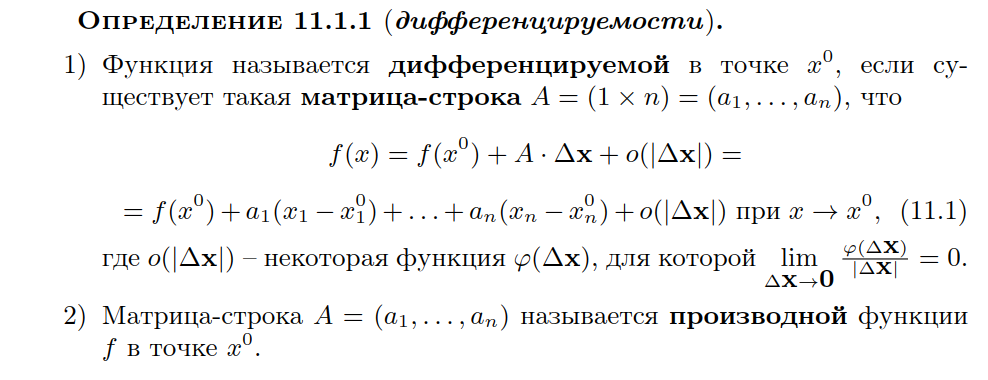
\includegraphics[width=\textwidth]{33.png}
    \vspace{-1.5cm}
\end{figure}

\begin{figure}[h!]
    \centering
    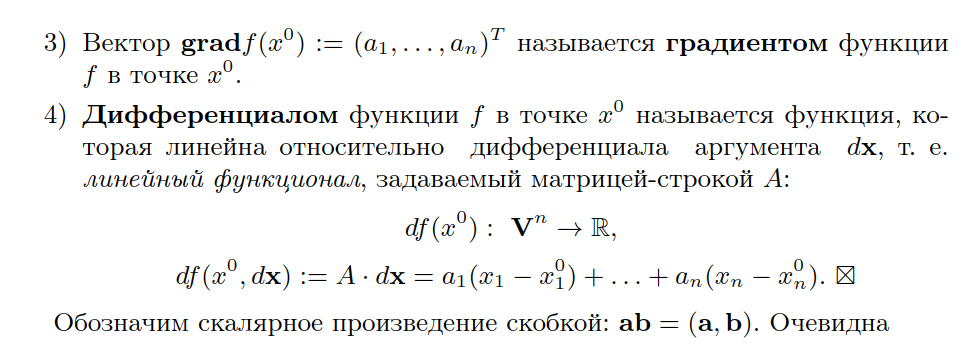
\includegraphics[width=\textwidth]{34.png}
    \vspace{-1cm}
\end{figure}
\begin{figure}[h!]
    \centering
    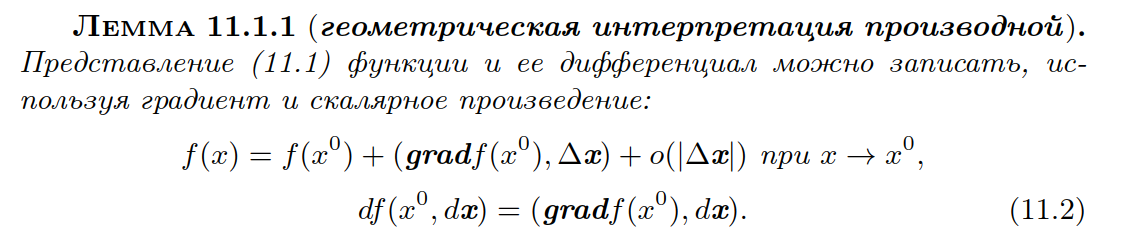
\includegraphics[width=\textwidth]{50.png}
    \vspace{-1cm}
\end{figure}

\newpage
\subsection{Частные производные функции нескольких переменных.}
\begin{figure}[h!]
    \centering
    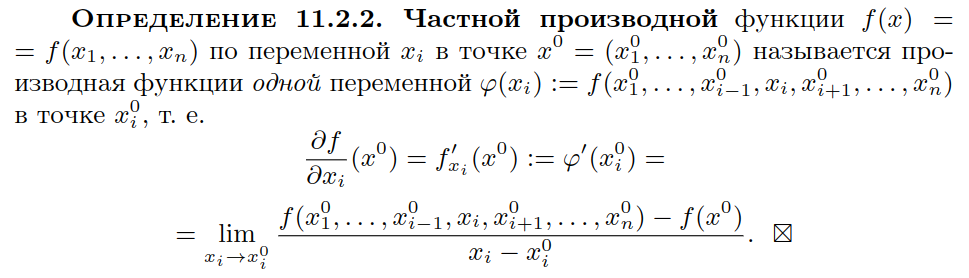
\includegraphics[width=\textwidth]{40.png}
    \vspace{-1.5cm}
\end{figure}

\begin{figure}[h!]
    \centering
    
\includegraphics[width=\textwidth]{35.png}
    \vspace{-1cm}
\end{figure}

\paragraph*{Лемма} Cуществует частная производная $\partial f(x^0)/\partial x_i$ $\Leftrightarrow$ $\exists \partial f(x^0)/\partial \mathbf{e}_i, \partial f(x^0)/\partial \mathbf{e}_i = \partial f(x^0)/\partial x_i$ где $\mathbf{e}_i$ -- базисный вектор.

\newpage
\subsection{Необходимые условия дифференцируемости, достаточные условия дифференцируемости функции нескольких переменных.}
\begin{figure}[h!]
    \centering
    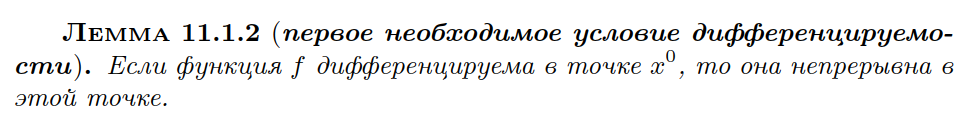
\includegraphics[width=\textwidth]{36.png}
    \vspace{-1cm}
\end{figure}

\begin{figure}[h!]
    \centering
    
\includegraphics[width=\textwidth]{37.png}
    \vspace{-1cm}
\end{figure}
\paragraph*{Пример} Парабола, поднятая вверх на 1, в точке (0,0) равна 0. Тогда производная по любому направлению равна нулю, но функция не непрерывна, значит не дифференцируема (по первому необходимому условию).

\begin{figure}[h!]
    \centering
    
\includegraphics[width=\textwidth]{38.png}
    \vspace{-1cm}
\end{figure}

\begin{figure}[h!]
    \centering
    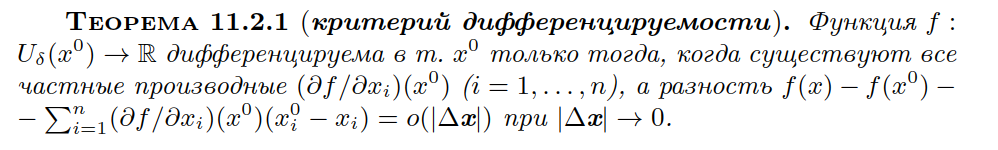
\includegraphics[width=\textwidth]{39.png}
    \vspace{-1cm}
\end{figure}

\newpage
\subsection{Дифференцируемость сложной функции.}

\newpage
\subsection{Инвариантность формы дифференциала относительно заменных.}

\newpage
\subsection{Градиент и производная по направлению.}
\begin{figure}[h!]
    \centering
    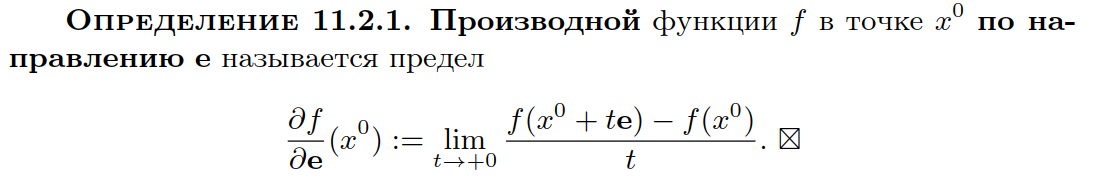
\includegraphics[width=\textwidth]{51.png}
    \vspace{-1cm}
\end{figure}

\newpage
\subsection{Не вошло в программу экзамена}
\subsubsection{Геометрический смысл градиента и частных производных}
\bb{Опр} $N$ -- ненулевой вектор в $V^p$. Множество точек $\R^p$, которое задаётся линейным уравнением $(N, x-x^0) = 0$ называется гиперплосколстью, проходящей через $x^0$ с вектором нормали $N$. Размерность гиперплоскости равна $p-1$.
\bb{Опр} Пусть $f$ дифференцируема в точке $x^0$. Гиперплоскость в пространстве $\R^{n+1}$, проходящая через точку $f(x^0)$ с вектором номрали $N = (gradf(x_0), - 1)$ называется касательной плоскостью к графику функции $f$ в точке $A(x^0, f(x^0))$
\paragraph*{Уравнение касательной плоскости}
$$ y = f(x^0) + (\x{grad} \, f(x^0), x-x^0) $$
\bb{Th} О касательной плоскости к графику.
\begin{enumerate}
    \item Касательная плоскоость -- единственная, которая проходит через точку касания и отличается от графика на величину бесконечно малую более высокого порядка, чем первый.
    \item Вектор $\x{grad}\, f$ если он отличен от нулевого, показывает направление максимального роста $f$, а $-\x{grad} \, f$ -- максимального убывания $f$
\end{enumerate}
\bb{Опр} Поверхностью уровня $c \in \R$ функции $f$ называется полный прообраз $f^{-1}(c) = \{ f(x) = c \}$. В типичной ситуации поверхность уровня -- это гипреповеръность рахмерности $n-1$.
\paragraph*{Пример} $f(x_1, x_2, x_3) = x_1^2 + x_2^2 + x_3^2$. Поверхнсть отрицательного уровня -- пустое множество, поврехность уровня 0 = $O(0,0,0)$, поверхность уровня $c>0$ -- сфера $x_1^2 + x_2^2+ x_3^2 = \sqrt{c}$.

\newpage
\subsection{Замечания и примеры}
\subsubsection{Треугольник диф, сущ чп, непр}
\begin{enumerate}
    \item $f$ -- дифференцируема $\Rightarrow$ $f$ имеет частные производные.
    \item $f$ -- дифференцируема $\Rightarrow$ $f$ непрерывна.
\end{enumerate}
\ii{Других логических соотношений между этими тремя фактами нет.}
\paragraph*{Контрпример 1}
\begin{equation*}
    f(x,y) = \left\{
    \begin{aligned}
         & \frac{2xy}{\sqrt{x^2 + y^2}}, \; (x,y) \neq (0,0) \\
         & 0, \; (x,y) = (0,0)
    \end{aligned}
    \right.
\end{equation*}
У неё есть частные производные и она непрерывна.

Из определения дифференцируемости:
$$\frac{f(x,y)}{\sqrt{x^2+y^2}} = \frac{2xy}{x^2 + y^2} = \sin{2\varphi} \nrightarrow 0, \rho \rightarrow 0; $$
Значит не дифференцируема.

\newpage
\section{Частные производные высших порядков, формула Тейлора.}
\subsection{Частные производные высших порядков.}

\newpage
\subsection{Независимость смешанной частной производной от порядка дифференцирования.}

\newpage
\subsection{Дифференциалы высших порядков.}

\newpage
\subsection{Формула Тейлора для функций нескольких переменных с остаточным членом в формах Лагранжа и Пеано.}

\newpage
\section{Жордан?}

\newpage
\section{Лебег?}

\newpage
\section{Определённые интегралы.}
\begin{figure}[h!]
    \centering
    \includegraphics[width=\textwidth]{52.png}
    \vspace{-1cm}
\end{figure}
\begin{figure}[h!]
    \centering
    \includegraphics[width=\textwidth]{53.png}
    \vspace{-1cm}
\end{figure}
\newpage
\begin{figure}[h!]
    \centering
    \includegraphics[width=\textwidth]{56.png}
    \vspace{-1cm}
\end{figure}
\begin{figure}[h!]
    \centering
    \includegraphics[width=\textwidth]{59.png}
    \vspace{-1cm}
\end{figure}
Ограниченная функция не всегда интегрируема, пример -- функция Дирихле. Нижний интеграл не будет равен верхнему.
\begin{figure}[h!]
    \centering
    \includegraphics[width=\textwidth]{61.png}
    \vspace{-1cm}
\end{figure}
\begin{figure}[h!]
    \centering
    \includegraphics[width=\textwidth]{62.png}
    \vspace{-1cm}
\end{figure}
\newpage
\subsection{Свойства сумм Дарбу}
\begin{figure}[h!]
    \centering
    \includegraphics[width=\textwidth]{54.png}
    \vspace{-1cm}
\end{figure}
\begin{figure}[h!]
    \centering
    \includegraphics[width=\textwidth]{55.png}
    \vspace{-1cm}
\end{figure}
\begin{figure}[h!]
    \centering
    \includegraphics[width=\textwidth]{57.png}
    \vspace{-1cm}
\end{figure}
\begin{figure}[h!]
    \centering
    \includegraphics[width=\textwidth]{58.png}
    \vspace{-1cm}
\end{figure}
\newpage
\subsection{Интегрируемость непрерывной функции, монотонной функции, ограниченной функции с конечным числом точек разрыва.}
\begin{figure}[h!]
    \centering
    \includegraphics[width=\textwidth]{60.png}
    \vspace{-1cm}
\end{figure}
\begin{figure}[h!]
    \centering
    \includegraphics[width=\textwidth]{67.png}
    \vspace{-1cm}
\end{figure}
\newpage
\subsection{Аддитивность интеграла по отрезкам, линейность интеграла, интегрируемость произведения функций, интегрируемость модуля интегрируемой функции, интегрируемость неравенств, теорема о среднем.}
\begin{figure}[h!]
    \centering
    \includegraphics[width=\textwidth]{65.png}
    \vspace{-1cm}
\end{figure}
\begin{figure}[h!]
    \centering
    \includegraphics[width=\textwidth]{66.png}
    \vspace{-1cm}
\end{figure}
\begin{figure}[h!]
    \centering
    \includegraphics[width=\textwidth]{68.png}
    \vspace{-1cm}
\end{figure}
\begin{figure}[h!]
    \centering
    \includegraphics[width=\textwidth]{69.png}
    \vspace{-1cm}
\end{figure}


\newpage
\subsection{Свойства интеграла с переменным верхним пределом -- непрерывность, дифференцируемость.}

\newpage
\subsection{Формула Ньютона-Лейбница}

\newpage
\subsection{Замена переменных и интегрирование по частям в определённом интеграле.}

\newpage
\subsection{Не вошло в программу экзамена}
\subsubsection{Необходимое условие существования интеграла Римана}
\vspace{-0.5cm}
\begin{figure}[h!]
    \centering
    \includegraphics[width=\textwidth]{63.png}
    \vspace{-1cm}
\end{figure}
\subsubsection{Эквивалентность Дарбу и Римана}
\begin{figure}[h!]
    \centering
    \includegraphics[width=\textwidth]{64.png}
    \vspace{-1cm}
\end{figure}



\newpage
\section{Неопределённые интегралы}
\begin{itemize}
    \item \textbf{Замена переменной}
          \begin{equation*}
              \int\frac{dx}{\sqrt{e^x+1}} = \left|
              \begin{aligned}
                   & t = e^x-1    \\
                   & x = \ln(t+1)
              \end{aligned} \right| = \int\frac{dt}{\sqrt{t}(t+1)} = \left|
              \begin{aligned}
                   & u = \sqrt{t} \\
                   & t = u^2
              \end{aligned} \right| = \int\frac{2udu}{u(u^2+1)}
          \end{equation*}
    \item \textbf{Интегрирование по частям}
          \begin{equation*}
              \int u v'dx = uv - \int u' v dx
          \end{equation*}
    \item \textbf{Рациональные функции}
          $$\int\frac{P(x)}{Q(x)}dx $$
          \begin{enumerate}
              \item $\deg P \geq \deg Q \Rightarrow$ выделить целую часть
              \item Разложтить знаменатель на неприводимые множители
              \item Представить $P/Q$ в виде суммы
              \item Найти неопределённые коэффициенты
              \item Проинтегрировать каждое слагаемое
          \end{enumerate}
    \item \textbf{Метод Остроградского}
          $$ \int \frac{P}{Q}dx = \frac{P_1}{Q_1} + \int \frac{P_2}{Q_2}dx$$
          $Q_2$ произведение всех неприводимых множителей $Q$, $Q_1 = Q/Q_2$
          $$ \int\frac{x^3+x^2-4x+1}{(x^2+1)^2}dx = \frac{Ax + B}{x^2+1} + \int\frac{Cx + D}{x^2+1} $$
          Дальше дифференцируем и находим коэффициенты.
    \item \textbf{Иррациональности}
          \begin{enumerate}
              \item $R(\alpha,\beta, \gamma,\ldots) = {P(\alpha, \beta, \gamma, \ldots)}/{Q(\alpha, \beta, \gamma, \ldots)} $
                    \begin{multline*}
                        \int R\left(x, \left(\frac{ax + b}{cx+d}\right)^{p_1/q_1}, \left(\frac{ax + b}{cx+ d}\right)^{p_2/1_2}, \ldots \right)dx = \\ = \left|
                        \begin{aligned}
                             & t^N = \frac{ax+b}{cx+d}       \\
                             & N = \x{НОК}(q_1, q_2, \ldots)
                        \end{aligned} \right| = \ldots
                    \end{multline*}
              \item Дифференциальный бином
                    $$ \int x^m (ax^n+b)^pdx $$
                    \begin{enumerate}
                        \item $p$ -- целое $\Rightarrow$ $x = t^N, \; N = \x{НОК}(\x{зн}(m), \x{зн}(n))$
                        \item $(m+1)/{n}$ -- целое $\Rightarrow$ $ax^n+b = t^s, \; s=\x{зн}(p)$
                        \item ${(m+1)}/{n}+p$ -- целое $\Rightarrow$ $a + b x^{-n} = t^s, \; s=\x{зн}(p)$
                        \item В остальных случаях интеграл не берётся.
                    \end{enumerate}
              \item Подстановки Эйлера
                    $$ \int R\left(x, \sqrt{ax^2+bx+c}\right)dx $$
                    \begin{equation*}
                        \sqrt{ax^2+bx+c} = \left\{
                        \begin{aligned}
                             & \pm \sqrt{a}x \pm t, \; a > 0 \\
                             & \pm xt \pm \sqrt{c}, \; c > 0 \\
                             & (x-x_{1,2})t
                        \end{aligned}
                        \right.
                    \end{equation*}
              \item $P(x, \sqrt{p})/Q(x, \sqrt{p})$
                    $$ \frac{P(x, \sqrt{p})}{Q(x, \sqrt{p})} = R_1(x) + R_2(x) \frac{1}{\sqrt{p}} $$
                    $$ \int\frac{\widetilde{p}(x)}{\sqrt{p}}dx = \widetilde{Q}(x)\sqrt{p} + \lambda\int\frac{1}{\sqrt{p}}dx $$
          \end{enumerate}
    \item \textbf{Тригонометрия}
          \begin{enumerate}
              \item $\int (\sin^nx \cdot \cos^m x ) dx  = |m \x{--нечёт}| = \int (\sin^nx\cdot \cos^{2k}x)d(\sin x)$
              \item $$\int \frac{P(\sin x, \cos x)}{Q(\sin x, \cos x)} dx, \quad P,Q\x{-- однородные, } \deg Q = \deg P + 2$$
                    Поделить обе части на $\cos^2x$, прератив в тангенсы.
              \item $\deg Q - \deg P = 2k \Rightarrow $ домножить на $(\cos^2x + \sin^2 x)$
              \item Сделать степени чётными, увеличив угол в два раза.
                    \begin{equation*}
                        \int \frac{1- \sin x + \cos x}{1+ \sin x - \cos x} dx = \left|
                        \begin{aligned}
                             & x = 2t       \\
                             & u = \tg t    \\
                             & u = \tg(x/2)
                        \end{aligned} \right| = \bigintsss{\ddfrac{1 - \frac{2u}{1+u^2} + \frac{1 - u^2}{1 + u^2}}{1 + \ddfrac{2u}{1+u^2} - \frac{1-u^2}{1 + u^2}}\frac{2 du}{1 + u^2}}
                    \end{equation*}
          \end{enumerate}
\end{itemize}

\newpage
\section{Несобственные интегралы}
$$ \lim\limits_{\varepsilon \to 0+}\int\limits_{a+\varepsilon}^b f(x) dx = \int\limits_a^bf(x)dx $$
$\exists$ конечный $\Rightarrow$ сходится. В обратном случае расходится.
\paragraph*{Условие сходимости по Коши}
$$\forall \varepsilon > 0 \; \exists c < b: \forall c_1, c_2 \in(c,b) \hookrightarrow \left| \int\limits_{c_1}^{c_2}f(x)dx \right| < \varepsilon$$
$$\exists \varepsilon > 0 \; \forall c < b: \exists c_1, c_2 \in(c,b) : \left| \int\limits_{c_1}^{c_2}f(x)dx \right| \geq \varepsilon$$
\subsection{Знакопостоянная функция}
\paragraph*{Th} \textit{(Первый признак сравнения)} Пусть $f$ и $g$ интегрируемы на $\forall [a,b']\subset [a,b)$. Если $0 \leq f\leq g$ на $ [a,b) $
\begin{itemize}
    \item и $\int_a^b g(x)dx $ сходится, то $\int_a^b f(x)dx $ тоже сходится.
    \item $\int_a^b f(x)dx $ расходится $\Rightarrow$ $\int_a^b g(x)dx $ расходится.
\end{itemize}


\paragraph*{Th} \textit{(Второй признак сравнения)} Пусть $f$ и $g$ интегрируемы на $\forall [a,b']\subset [a,b)$. Если $ \lim\limits_{x\to b-0}{f(x)}/{g(x)} = k \in \R \neq 0$ то либо оба сходятся, либо оба расходятся.

В этом случае пишут $\int\limits_a^b f(x)dx \mathop{\sim}\limits^{\mathrm{\x{сх}}}\int\limits_a^bg(x) dx$
\subsection{Знакопеременная функция}
\paragraph*{Th} Если $\int_a^b |f(x)|dx$ сходится, то $\int_a^b f(x)dx $ сходится и $\int_a^b f(x)dx $ называется абсолютно сходящейся ($f$ абсолютно интегрируема).
\paragraph*{Th} Если $\int_a^b |f(x)|dx $ расходится, а $\int_a^b f(x)dx $ сходится, то $\int_a^b f(x) dx $ называется условно сходящейся ($f$ условно интегрируема). Если $\int_a^b f(x)dx $ расходится, то всё.
\newpage
\paragraph*{Th} $\int_a^bf(x)g(x)dx$ сходится, если:
\begin{table}[h!]
    \centering
    \begin{tabular}{|ll|}
        \hline
        \multicolumn{1}{|l|}{Дирихле}                                                   & Абель                                      \\ \hline
        \multicolumn{2}{|l|}{$f$ непрерывна, $g$ непрерывно дифференцируема и монотонна.}                                            \\ \hline
        \multicolumn{1}{|l|}{F(x) ограничена на $[a,b)$, $g(x)\xrightarrow{x\to  b} 0$} & $F \xrightarrow{x\to b} C$, $g$ ограничена \\ \hline
    \end{tabular}
\end{table}
\paragraph*{Выделение главной части} $f(x) = g(x) + R(x)$, $R(x)$ абсолютно интегрируема. Тогда $\int_a^b f(x)dx $ и $\int_a^bg(x)dx$:
\begin{itemize}
    \item Либо оба расходятся
    \item Либо оба сходятся условно
    \item Либо оба сходятся абсолютно
\end{itemize}
\paragraph*{Алгоритм}
\begin{enumerate}
    \item Абсолютная сходимость (сравнение, выделение главной части)
    \item Условная сходимость
          \begin{enumerate}
              \item $ \int f(x)dx $ сходится (Дирихле, Абель, главная часть)
              \item $ \int |f(x)|dx $ расходится (оценка, главная часть)
          \end{enumerate}
    \item Расходимость $ \int f(x) dx  $ (критерий Коши)
\end{enumerate}
\subsection{Шаблонные интегралы}
\begin{multicols}{2}
\begin{enumerate}
    \item $\int\limits_1^{+\infty}x^\alpha dx$ сходится $\Leftrightarrow \alpha < -1 $
    \item $\int\limits_1^{+\infty}1/x^\alpha dx$ сходится $\Leftrightarrow \alpha  > 1$
    \item $ \int\limits_0^1 1/x^\alpha dx $ сходится $\Leftrightarrow \alpha  < 1$
    \item $\int\limits_0^1 x^\alpha dx $ сходится $\Leftrightarrow \alpha > -1 $
    \item $\int\limits_2^{+\infty}x^\alpha \ln^\beta x dx$ Сходится, если: \\
    1. $ \alpha < -1 $ 2. $ \alpha = -1,\; \beta < -1 $
\end{enumerate}
\end{multicols}
$|\sin x|\geq \frac{2}{\pi}|x|$

\subsection{Примеры}
Исследовать на сходимость $\forall \alpha, \beta$ $\int\limits_2^{+\infty}x^\alpha \ln^\beta x dx$
\begin{enumerate}
    \item $\alpha < -1 $
            $$x^\alpha = x^{\frac{\alpha +1}{2}}\cdot x^\frac{\alpha - 1}{2}  $$
    Заметим, что $x^\frac{\alpha + 1}{2} \ln^\beta x \xrightarrow[x\to+\infty]{\alpha > -1} 0 \Rightarrow $ ограничена $\Rightarrow \exists C: x^\frac{\alpha + 1}{2} \leq C$ \
    $$ \int\limits_2^{+\infty} x^\alpha \ln^\beta x dx = \int\limits_2^{+\infty}x^\frac{\alpha - 1}{2} \cdot x^\frac{\alpha + 1}{2}\ln^\beta x dx \leq C\int\limits_2^{+\infty} x^\frac{\alpha -1}{2}dx$$
    Шаблонный, сходится тогда и только тогда, когда $\alpha < -1$
    \item $\alpha = -1$
    $$ \int\limits_2^{+\infty}\frac{\ln^\beta x}{x}dx = \int\limits_2^{+\infty}\ln^\beta x d(\ln x) =|\ln x = t| = \int\limits_{\ln 2}^{+\infty} t^\beta dt$$
    Сходистя, когда $\beta < -1$
    \item $\alpha > -1 $
    $$ \int\limits_2^{+\infty}x^\alpha \ln^\beta x dx = \int\limits_2^{+\infty} x^\frac{\alpha -1}{2}\cdot x^\frac{\alpha +1}{2}\ln^\beta x dx \geq C\int\limits_2^{+\infty} x^\frac{\alpha -1}{2}dx $$
    Расходится при $\alpha \geq -1$ $\Rightarrow$ Исходный расохдится при $\alpha > -1$ по признаку сравнения.
\end{enumerate}



\end{document}
